% !TEX program = pdflatex
% Mercury --- tesi di laurea
% Template ufficiale Universitas Mercatorum (report twoside/openright, Times, interlinea 1.5)
% Compila con:  latexmk -pdf main.tex
\documentclass[twoside,12pt,openright]{report}
\usepackage[utf8]{inputenc}
\usepackage[T1]{fontenc}
\usepackage[italian]{babel}
\usepackage[a4paper,top=3cm,bottom=3cm,left=3cm,right=3cm,marginparwidth=1.5cm,bindingoffset=15mm,heightrounded]{geometry}
\usepackage{csquotes}
\usepackage{quoting}
\quotingsetup{font=small}

% Times New Roman + interlinea 1.5 (mandatorie Mercatorum)
\usepackage{times}
\linespread{1.5}

% Box colorati (dal template)
\usepackage{tcolorbox}
\usepackage{mdframed}

\usepackage{amssymb}
\usepackage{amsmath}
\usepackage{graphicx}
\usepackage{booktabs}
\usepackage{microtype}

\usepackage[colorlinks=true, allcolors=black]{hyperref}

% Codice
\usepackage{xcolor}
\usepackage{colortbl}
\usepackage{array}
\usepackage{listings}

% Swift (usato nel capitolo Implementazione)
\lstdefinelanguage{Swift}{
  keywords={class,struct,enum,protocol,func,var,let,if,else,for,while,return,import,guard,switch,case,break,continue,in,as,is,nil,self,Self,init,deinit,private,public,internal,fileprivate,open,static,final,override,extension,do,try,catch,throws,async,await,actor,@Model,@Environment,@State,@Binding,@Observable},
  keywordstyle=\color{blue!70!black}\bfseries,
  comment=[l]{//},
  morecomment=[s]{/*}{*/},
  commentstyle=\color{gray}\itshape,
  stringstyle=\color{purple!70!black},
  morestring=[b]",
  sensitive=true
}
\lstset{basicstyle=\ttfamily\small,frame=single,breaklines=true,showstringspaces=false}

\usepackage[style=apa, backend=biber]{biblatex}
\addbibresource{refs.bib}

\begin{document}

\newgeometry{top=3cm,bottom=3cm,left=3cm,right=3cm,heightrounded}
\begin{titlepage}
    \begin{figure}[!htb]
        \centering
         
\includegraphics[keepaspectratio=true,scale=3.5]{Immagini/Mercatorum logo.jpg}
    \end{figure}

    \begin{center}
        \vspace{5mm}
        \large{\textbf{FACOLTÀ DI SCIENZE TECNOLOGICHE E DELL'INNOVAZIONE}}
        \vspace{1.5mm}

        \noindent\rule{225pt}{0.4pt}

        \vspace{5mm}

        \large{\textbf{CORSO DI LAUREA IN INGEGNERIA INFORMATICA (L-8)}}

        \vspace{10mm}

        \Large{\textbf{\emph{Prova Finale in}}}

        \large{\textbf{PROGRAMMAZIONE}}

        \vspace{1mm}

        \large{Mercurio --- Progettazione e implementazione di un'app iOS per
        l'aggregazione personalizzata di feed RSS italiani con integrazione di
        provider AI}

    \end{center}

    \vspace{15mm}

    \begin{minipage}[t]{0.33\textwidth}
        \centering
        {\large RELATORE\\[0.5em]
         \normalsize Chiar.mo\\
         Prof. Mauro Bellone}
    \end{minipage}
    \hfill
    \begin{minipage}[t]{0.35\textwidth}
        \centering
        {\large CANDIDATO\\[0.5em]
         \large Alessio Iodice\\[0.5em]
         \normalsize MATR. 0082301723}
    \end{minipage}

    \vspace{20mm}

    \centering{\normalsize{Anno Accademico 2025/2026}}

\end{titlepage}
\restoregeometry


\newpage
\null
\newpage

% ===================== Sommario =====================
\chapter*{Sommario}
\addcontentsline{toc}{chapter}{Sommario}
\input{Capitoli/_abstract.txt}

\vspace{1em}
\noindent\textbf{Codice sorgente.} Il repository del progetto è disponibile su
GitHub: \url{https://github.com/Yoddikko/Mercury}.

\tableofcontents

% ===================== Corpo (9 capitoli) =====================
\chapter{Introduzione}
\label{cap:introduzione}

\section{Contesto e motivazione}
Il consumo di notizie online vive due tensioni opposte. Da un lato la quantità
di contenuti pubblicati ogni giorno supera di molto la capacità di attenzione
di una persona. Dall'altro l'utente si ritrova frammentato su decine di
applicazioni proprietarie, ognuna con il proprio algoritmo opaco e con poco
controllo sulle fonti. RSS, pur tecnicamente datato, resta l'unico standard
aperto che lascia all'utente la scelta esplicita delle fonti e la lettura in un
unico luogo.

Nel frattempo i modelli linguistici di grandi dimensioni (LLM) hanno reso
economicamente sostenibile l'arricchimento automatico dei contenuti editoriali:
sintesi, categorizzazione, clustering. Gli aggregatori commerciali attuali
hanno però due limiti. L'arricchimento è spesso opaco e legato a un singolo
fornitore, e i dati di interazione finiscono in cloud anche quando non ce ne
sarebbe bisogno.

Mercury nasce per esplorare un punto intermedio: un aggregatore RSS nativo iOS
in cui (i) la persistenza è locale per impostazione predefinita, (ii) l'utente
sceglie quale provider AI usare e con quali credenziali, e (iii) sintesi e
categorizzazione sono trasparenti, etichettate e disattivabili.

\section{Obiettivi}
La tesi persegue cinque obiettivi tra loro complementari:
\begin{enumerate}
  \item progettare un'architettura modulare iOS che separi presentazione,
        dominio, persistenza e integrazioni AI in layer testabili;
  \item realizzare una pipeline RSS robusta capace di ingestire, normalizzare
        e deduplicare articoli da fonti eterogenee;
  \item integrare cinque provider AI (OpenAI, Anthropic, Google, Ollama, DeepSeek)
        dietro un'unica astrazione, con configurazione utente;
  \item garantire una persistenza locale-first con SwiftData per supportare
        l'uso offline e la privacy;
  \item formalizzare e validare un \textbf{processo di sviluppo agentico}
        documentato, con tracciabilità completa issue\,$\to$\,branch\,$\to$\,PR\,$\to$\,merge,
        come contributo metodologico oltre al manufatto software.
\end{enumerate}

\section{Struttura del documento}
Il documento segue la catena ingegneristica classica~\cite{sommerville2016}
richiesta dal relatore. Il
Cap.~\ref{cap:stato-arte} delinea lo stato dell'arte. Il
Cap.~\ref{cap:requisiti} formalizza requisiti funzionali e non funzionali con
identificatori tracciabili. Il Cap.~\ref{cap:specifiche} traduce i requisiti in
specifiche architetturali e di dominio. Il Cap.~\ref{cap:progettazione}
contiene il modello UML, lo schema dati e i diagrammi di sequenza. Il
Cap.~\ref{cap:metodologia} è il contributo distintivo della tesi: descrive
toolchain, governance documentale e riflessione critica
sull'approccio agentico. Il Cap.~\ref{cap:implementazione} riporta le scelte
implementative non banali con riferimento alle issue e ai PR del repository. Il
Cap.~\ref{cap:testing} discute strategia e copertura dei test, mentre il
Cap.~\ref{cap:conclusioni} sintetizza risultati, limiti e sviluppi futuri.

\section{Glossario minimo}
\label{sec:glossario}
Termini ricorrenti nel documento, definiti una volta sola.

\begin{description}
  \item[Outlet / testata] Una fonte giornalistica del catalogo (es.
        ANSA, Corriere). Un outlet può esporre più feed RSS (sezioni).
  \item[Feed RSS] Il file XML pubblicato da una testata con l'elenco
        degli ultimi articoli (titolo, link, riassunto, data).
  \item[Ingest] Il momento in cui l'app scarica i feed e salva gli
        articoli in locale.
  \item[Enrichment] Il passo successivo all'ingest: l'app scarica la
        pagina web dell'articolo per ricavarne il testo completo,
        perché il feed di solito contiene solo un estratto.
  \item[Chrome / boilerplate] Tutto ciò che nella pagina web non è
        articolo: banner cookie, menu, box ``Leggi anche'', pulsanti
        di condivisione, inviti all'abbonamento.
  \item[Distillazione] La pulizia automatica della pagina: dal
        HTML completo si estrae il solo corpo dell'articolo,
        eliminando il chrome. È una pipeline a stadi successivi.
  \item[Pipeline] Una catena di passi applicati in sequenza allo
        stesso dato; l'output di un passo è l'input del successivo.
  \item[CTA] \emph{Call to action}: testo o pulsante che invita
        l'utente a fare qualcosa (``Abbonati'', ``Accetta i cookie'').
  \item[Teaser] L'anteprima gratuita di un articolo a pagamento:
        poche righe seguite dall'invito ad abbonarsi.
  \item[Fixture] Una pagina HTML reale salvata nel repository e usata
        nei test: la pipeline viene rieseguita su di essa a ogni build
        per accorgersi subito di eventuali regressioni.
  \item[Readability] Algoritmo open source di Mozilla (usato dalla
        modalità lettura di Firefox e da molte app di lettura) che
        individua il corpo di un articolo dentro una pagina web.
  \item[Purge / retention] Pulizia della cache locale: \emph{purge} =
        cancellare subito ciò che non serve più; \emph{retention} =
        conservare i dati solo per un periodo massimo (qui 30 giorni).
\end{description}

% =============================================================
\chapter{Stato dell'arte}
\label{cap:stato-arte}

\section{Aggregatori di feed esistenti}
Il segmento degli aggregatori RSS è dominato da pochi prodotti consolidati.
\emph{Feedly} offre sincronizzazione cloud, categorizzazione automatica e da
qualche anno una funzione di sintesi basata su LLM (Feedly~AI) disponibile
nelle fasce a pagamento~\cite{feedly}. \emph{NetNewsWire} è un client open
source per Apple~\cite{netnewswire}, strettamente locale, privo di funzioni AI
integrate. \emph{Reeder} è un client
commerciale focalizzato sulla qualità di lettura e sulla compatibilità con
servizi di sincronizzazione di terze parti (iCloud, Feedbin, Inoreader). Ne
emerge una separazione netta tra ``letture pulite ma senza intelligenza''
(NetNewsWire, Reeder) e ``intelligenza opaca lato cloud'' (Feedly). Mercury si
colloca in mezzo: letture pulite locali, arricchimento AI esplicito e
configurabile.

\section{Tecniche di clustering di notizie}
La letteratura sul clustering di notizie include sia approcci industriali
proprietari sia sistemi accademici. \emph{Google News} costruisce
\emph{storylines} aggregando articoli su uno stesso evento attraverso
similarità testuale e segnali temporali. Sistemi accademici come
\emph{NewsClusterer} e variazioni di Louvain~\cite{blondel2008louvain} o
HDBSCAN~\cite{campello2013hdbscan} su embedding densi
mostrano che il clustering online (incrementale, su singolo articolo in arrivo)
è praticabile su volumi medi.

Tre sono le scelte che contano: la rappresentazione (TF-IDF contro embedding
neurale), la metrica di similarità (la cosine è lo standard de facto~\cite{manning2008ir})
e la soglia di assegnazione. Mercury adotta la specifica per un clustering
opzionale basato su embedding e cosine similarity con soglia 0,75, come
documentato in \texttt{docs/features/CLUSTERING.md}. L'implementazione è
rimandata a fasi successive del progetto.

\section{Personalizzazione on-device}
La personalizzazione di contenuti su dispositivo attira interesse crescente
perché evita il trasferimento di segnali comportamentali sensibili.
Apple ha introdotto framework dedicati (\emph{Core~ML}, \emph{Create~ML},
\emph{Natural~Language})~\cite{apple-coreml} che consentono inferenza locale su
modelli moderatamente grandi. Per task ``leggeri'' come il ranking di un feed personale
(centinaia di articoli, decine di feature) un punteggio lineare locale basta e
avanza, e ha il vantaggio di restare ispezionabile.

Il principio guida è \emph{local-first}~\cite{kleppmann2019localfirst}: i dati
di interazione restano sul dispositivo, la sincronizzazione cloud è opt-in. Mercury vi aderisce:
SwiftData è la sorgente di verità, Firebase è citato come opzione
futura per la sincronizzazione cross-device.

\section{LLM applicati a contenuti editoriali}
L'uso di LLM per sintesi, categorizzazione e classificazione di testi
giornalistici è ormai consolidato. I rischi documentati sono soprattutto le
allucinazioni (introduzione di fatti non presenti nel testo
originale)~\cite{ji2023hallucination}, il bias
del modello e la dipendenza da un singolo fornitore commerciale. Le mitigazioni
accettate includono prompt deterministici con vincoli espliciti
(``usa solo il contenuto fornito''), output JSON validati lato client, e
astrazione del fornitore dietro un'interfaccia comune così da poter migrare o
duplicare senza riscrivere la logica applicativa.

Sono esattamente le mitigazioni che Mercury adotta: prompt versionati
(\texttt{docs/ai/PROMPTS.md}), astrazione \texttt{AIProvider} (PR~\#23) e
quattro implementazioni intercambiabili.

\section{Confronto sintetico}
La Tab.~\ref{tab:confronto-aggregatori} riassume il posizionamento di Mercury
rispetto agli aggregatori principali, lungo le dimensioni rilevanti per gli
obiettivi del progetto.

\begin{table}[h]
\centering
\small
\caption{Confronto sintetico tra Mercury e gli aggregatori RSS principali.}
\label{tab:confronto-aggregatori}
\begin{tabular}{lcccc}
\toprule
\textbf{Dimensione} & \textbf{Feedly} & \textbf{NetNewsWire} & \textbf{Reeder} & \textbf{Mercury} \\
\midrule
Open source                    & no  & sì  & no  & sì (MIT) \\
Storage primario               & cloud & locale & locale & locale \\
Sintesi AI integrata           & sì (a pagamento) & no & no & sì (on-demand) \\
Categorizzazione AI            & sì (opaca) & no & no & sì (etichettata) \\
Provider AI scegli\-bile dall'utente & no & --- & --- & sì (5 provider) \\
Clustering eventi              & parziale & no & no & specificato (futuro) \\
Funziona offline               & limitato & sì & sì & sì \\
Etichettatura contenuto AI     & parziale & --- & --- & richiesta \\
\bottomrule
\end{tabular}
\end{table}

% =============================================================
\chapter{Analisi dei requisiti}
\label{cap:requisiti}

\section{Requisiti funzionali}
I requisiti funzionali sono numerati e prioritizzati secondo lo schema
MoSCoW~\cite{dsdm2014moscow} (M = Must, S = Should, C = Could). La priorità riflette lo scope per la
versione MVP della tesi.

\begin{table}[h]
\centering
\small
\caption{Requisiti funzionali (RF).}
\label{tab:rf}
\begin{tabular}{p{1.2cm}p{10cm}p{1cm}p{1.5cm}}
\toprule
\textbf{ID} & \textbf{Descrizione} & \textbf{Pri.} & \textbf{Cap.} \\
\midrule
RF-1  & Il sistema deve scaricare feed RSS/Atom da un catalogo di sorgenti predefinite. & M & \ref{cap:implementazione} \\
RF-2  & Il sistema deve effettuare il parsing dei feed scaricati estraendo metadati estesi (titolo, link, autore, data, immagine, lingua, categorie). & M & \ref{cap:implementazione} \\
RF-3  & Il sistema deve normalizzare gli articoli in un modello di dominio unico e deduplicare per URL. & M & \ref{cap:implementazione} \\
RF-4  & Il sistema deve persistere gli articoli normalizzati in modo locale e offline. & M & \ref{cap:implementazione} \\
RF-5  & Il sistema deve esporre un feed di articoli in ordine cronologico inverso come comportamento di fallback. & M & \ref{cap:implementazione} \\
RF-6  & L'utente deve poter aprire il dettaglio di un articolo e accedere al corpo completo. & M & \ref{cap:implementazione} \\
RF-7  & Se il corpo RSS appare incompleto, il sistema deve effettuare un best-effort di estrazione dalla pagina HTML originale. & S & \ref{cap:implementazione} \\
RF-8  & L'utente deve poter salvare (bookmark) un articolo. & S & \ref{cap:implementazione} \\
RF-9  & Il sistema deve esporre un Developer Playground in modalità debug per diagnostica dei feed. & S & \ref{cap:implementazione} \\
RF-10 & Il sistema deve fornire un layer AI plug-in compatibile con almeno cinque provider (OpenAI, Anthropic, Google, Ollama, DeepSeek). & M & \ref{cap:implementazione} \\
RF-11 & L'utente deve poter selezionare provider, modello e fornire la propria API key tramite Keychain. & M & \ref{cap:implementazione} \\
RF-12 & Il sistema deve generare una sintesi (corta + bullet) di un articolo su richiesta utente. & S & \ref{cap:implementazione} \\
RF-13 & Il sistema deve categorizzare un articolo (categoria singola + tag multipli) su richiesta. & S & \ref{cap:implementazione} \\
RF-14 & Ogni contenuto generato da AI deve essere etichettato come tale nell'interfaccia. & M & \ref{cap:implementazione} \\
RF-15 & Il sistema deve memorizzare preferenze utente (categorie, topic, fonti preferite, fonti nascoste, lingua). & S & \ref{cap:specifiche} \\
RF-16 & Il sistema deve produrre un feed personalizzato ordinato per punteggio (recency, match categoria, match topic, engagement, preferenza fonte). & C & \ref{cap:implementazione} \\
RF-17 & Il sistema deve poter raggruppare articoli sullo stesso evento (cluster) tramite similarità su embedding. & C & \ref{cap:implementazione} \\
RF-18 & Il sistema deve emettere log strutturati esportabili in modalità debug. & M & \ref{cap:implementazione} \\
RF-19 & L'interfaccia deve essere localizzata in almeno italiano e inglese. & M & \ref{cap:implementazione} \\
RF-20 & Il sistema deve esporre un'esportazione testuale dello stato delle sorgenti (outlets report). & C & \ref{cap:implementazione} \\
RF-21 & Il sistema deve offrire un feed personalizzato basato sugli interessi dichiarati dall'utente, classificato tramite il provider AI configurato, con stati espliciti in assenza di provider o di interessi. & S & \ref{cap:implementazione} \\
\bottomrule
\end{tabular}
\end{table}

\section{Requisiti non funzionali}
\begin{table}[h]
\centering
\small
\caption{Requisiti non funzionali (RNF).}
\label{tab:rnf}
\begin{tabular}{p{1.2cm}p{3cm}p{9.5cm}}
\toprule
\textbf{ID} & \textbf{Categoria} & \textbf{Vincolo} \\
\midrule
RNF-1  & Prestazioni     & Il rendering della home non deve bloccare il main thread; le operazioni di rete e AI devono essere asincrone (async/await). \\
RNF-2  & Prestazioni     & La lettura del feed da cache locale deve essere percepita come istantanea ($<$100\,ms per centinaia di articoli). \\
RNF-3  & Privacy         & Nessun dato di interazione utente lascia il dispositivo per impostazione predefinita. La sincronizzazione cloud è opt-in. \\
RNF-4  & Sicurezza       & Le API key dei provider AI devono essere memorizzate in Keychain, mai in chiaro su disco. \\
RNF-5  & Sicurezza       & I log non devono contenere segreti, token o contenuto utente privato. \\
RNF-6  & Offline         & Articoli, sintesi, categorie e preferenze già acquisite devono essere disponibili offline. \\
RNF-7  & Accessibilità   & Tutti i controlli interattivi devono avere etichette di accessibilità localizzate. \\
RNF-8  & Localizzazione  & Le stringhe rivolte all'utente non devono essere hard-coded; uso obbligatorio dei file di localizzazione. \\
RNF-9  & Manutenibilità  & Architettura MVVM rispettata; nessuna chiamata a provider AI direttamente da Views/ViewModels. \\
RNF-10 & Osservabilità   & Ogni funzione nuova o modificata deve emettere log via \texttt{AppLogger}; propagazione del request id nei flussi multi-layer. \\
RNF-11 & Robustezza      & Nessun fallimento silenzioso: errori RSS, AI o persistenza devono produrre log e fallback. \\
RNF-12 & Portabilità     & Target iOS~17+, Swift~5.9+, dipendenze esterne minime (SwiftData, SwiftUI nativi). \\
\bottomrule
\end{tabular}
\end{table}

\section{Casi d'uso}
La Fig.~\ref{fig:usecase} riassume i casi d'uso del sistema. Le tabelle che
seguono descrivono i quattro scenari principali.

\begin{figure}[h]
\centering
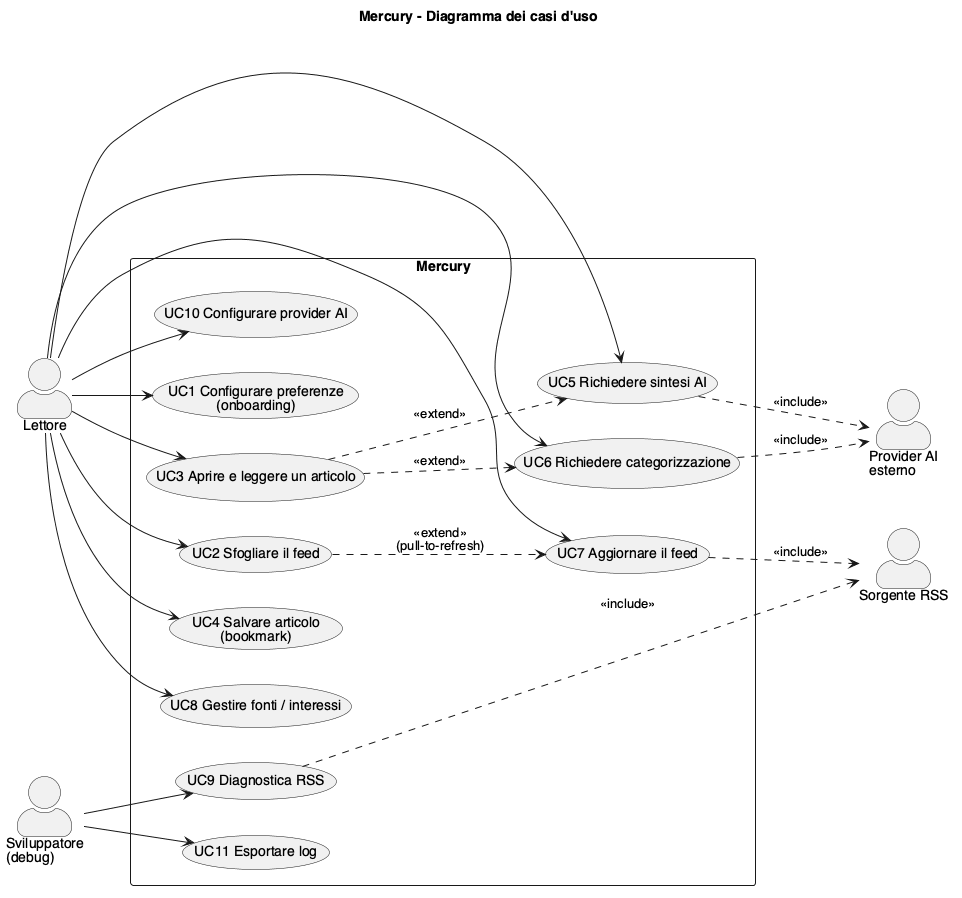
\includegraphics[width=0.9\textwidth]{figures/usecase.png}
\caption{Diagramma dei casi d'uso di Mercury.}
\label{fig:usecase}
\end{figure}

\subsection*{UC1: configurazione preferenze (onboarding)}
\textbf{Attore:} lettore (primo avvio).\\
\textbf{Pre:} app installata, nessun profilo locale.\\
\textbf{Flusso principale:} quattro passi. Introduzione alle funzioni,
selezione delle testate italiane (senza scaricare articoli), scelta degli
interessi (etichette suggerite più campo libero), configurazione facoltativa
del provider AI.\\
\textbf{Post:} esiste un \texttt{UserPreferenceEntity} locale con
\texttt{hasCompletedOnboarding} attivo; il primo download parte solo dopo la
conferma finale.\\
\textbf{Tracciabilità:} RF-15, RF-19, RF-21.

\subsection*{UC2: lettura del feed}
\textbf{Attore:} lettore.\\
\textbf{Flusso principale:} apertura Home, caricamento articoli da SwiftData,
visualizzazione in lista, pull-to-refresh facoltativo (estende UC7). La Home
offre tre viste: cronologica, per argomenti (sez.~\ref{sec:topic-feed}) e
personalizzata ``Per~te'' (sez.~\ref{sec:personalization}).\\
\textbf{Variante:} senza interessi o senza provider AI configurato la vista
``Per~te'' mostra uno stato dedicato; il fallback resta il feed cronologico
(RF-5).\\
\textbf{Tracciabilità:} RF-4, RF-5, RF-16, RF-21.

\subsection*{UC3: sintesi AI di un articolo}
\textbf{Attore:} lettore + provider AI esterno.\\
\textbf{Pre:} articolo aperto, AI configurata, connettività disponibile.\\
\textbf{Flusso principale:} richiesta sintesi, costruzione prompt, chiamata
provider, validazione output JSON, persistenza locale, render con etichetta
``generato da AI''.\\
\textbf{Eccezioni:} provider non configurato $\to$ stato vuoto con messaggio;
errore provider $\to$ log e UI non bloccante.\\
\textbf{Tracciabilità:} RF-10, RF-11, RF-12, RF-14.

\subsection*{UC4: salvataggio articolo}
\textbf{Attore:} lettore.\\
\textbf{Flusso principale:} tap su pulsante bookmark, aggiornamento campo
\texttt{isBookmarked} su \texttt{ArticleEntity}, visibilità persistente offline.\\
\textbf{Tracciabilità:} RF-8.

\section{Vincoli e ipotesi}
\begin{itemize}
  \item Target tecnologico: iOS~17+, Swift~5.9+, SwiftData, SwiftUI.
  \item Approccio local-first: la fonte di verità è on-device; il cloud è
        opzionale e non richiesto dall'MVP.
  \item L'utente fornisce le proprie credenziali API. Mercury non distribuisce
        token né opera un backend proxy nella versione MVP.
  \item I provider AI sono assunti remoti (eccetto Ollama, locale). La
        latenza è gestita tramite operazioni asincrone e non blocca la lettura.
  \item Il clustering semantico su embedding è specificato come
        obiettivo; l'MVP ne implementa un'approssimazione lessicale
        on-device (sez.~\ref{sec:topic-feed}).
\end{itemize}

\paragraph{Tracciabilità.} Ogni RF è ricondotto al capitolo che lo realizza
nella colonna \emph{Cap.} di Tab.~\ref{tab:rf}. Le specifiche del
Cap.~\ref{cap:specifiche} dettagliano i componenti che soddisfano i requisiti;
il Cap.~\ref{cap:implementazione} cita le issue e i PR specifici (es. RF-1/2/3
$\to$ PR~\#16, \#22, \#38; RF-4 $\to$ PR~\#24, \#35, \#37;
RF-5 $\to$ PR~\#36; RF-6/8 $\to$ PR~\#35, \#40; RF-9 $\to$ PR~\#15, \#20, \#41;
RF-10/11 $\to$ PR~\#23, \#39, \#42;
RF-15 $\to$ PR~\#24, \#34; RF-18 $\to$ PR~\#19).

% =============================================================
\chapter{Specifiche}
\label{cap:specifiche}

\section{Architettura logica}
Mercury adotta MVVM con SwiftUI~\cite{apple-swiftui} per la presentazione, una application layer di
use case che orchestra i servizi di dominio, una data layer che isola
persistenza e networking, e una AI layer plug-in che astrae i provider esterni.
La Fig.~\ref{fig:architecture} riporta i componenti principali e le loro
dipendenze.

\begin{figure}[h]
\centering
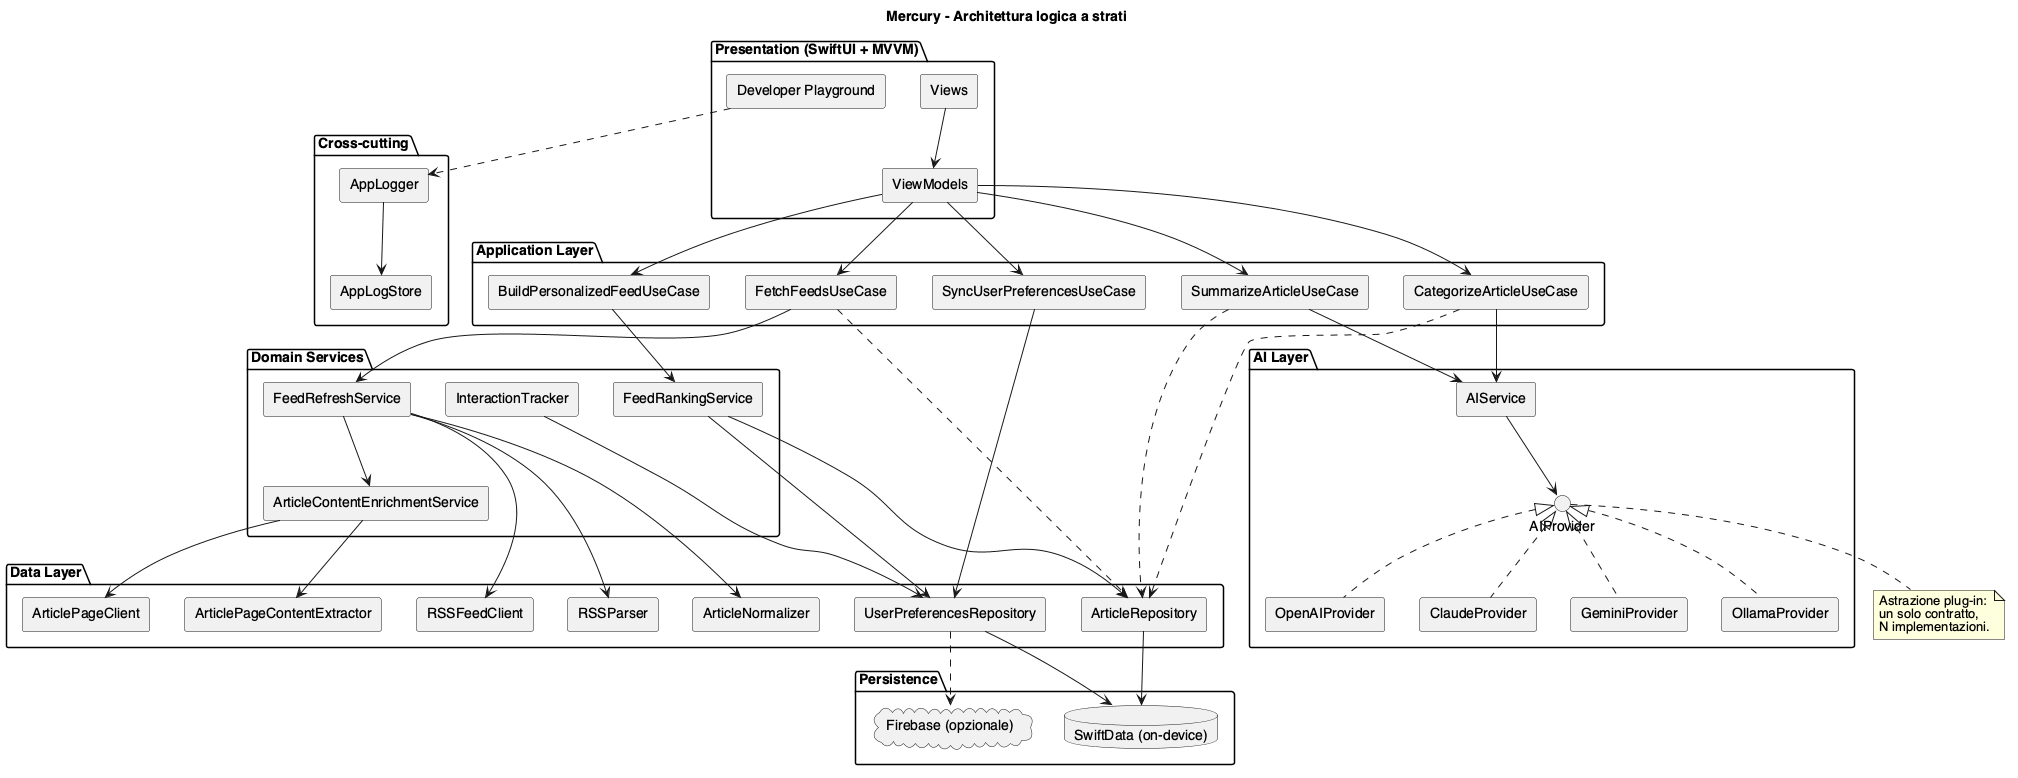
\includegraphics[width=\textwidth]{figures/architecture.png}
\caption{Architettura logica di Mercury (componenti e dipendenze).}
\label{fig:architecture}
\end{figure}

\paragraph{Principi di separazione.}
\begin{itemize}
  \item le View non contengono logica di parsing, rete o persistenza;
  \item i ViewModel non chiamano direttamente i provider AI;
  \item ogni use case incapsula uno scenario applicativo e orchestra
        repository e servizi;
  \item l'unico punto di ingresso verso un provider AI è \texttt{AIService},
        che non effettua fallback automatici (fail-fast).
\end{itemize}

\section{Modello del dominio}
Il modello di dominio è composto da quattro entità persistenti.

\paragraph{\texttt{ArticleEntity}.} È un articolo normalizzato.
Campi chiave: \texttt{id} (hash dell'URL), \texttt{title}, \texttt{sourceName},
\texttt{sourceURL}, \texttt{articleURL}, \texttt{publishedAt}, \texttt{rawContent},
\texttt{cleanedContent}, \texttt{summaryShort}, \texttt{summaryBullets},
\texttt{category}, \texttt{tags}, \texttt{language}, \texttt{isBookmarked},
\texttt{isRead}, \texttt{clusterID}, \texttt{createdAt}, \texttt{updatedAt}.
È la \emph{single source of truth} per il contenuto. Tutti i campi AI sono
opzionali e popolati in modo asincrono e incrementale.

\paragraph{\texttt{ClusterEntity}.} È un evento, cioè un gruppo di
articoli che parlano della stessa notizia. Campi: \texttt{id}, \texttt{title},
\texttt{summary}, \texttt{mainTopic}, \texttt{articleIDs}, \texttt{createdAt}.
Un articolo può appartenere ad al più un cluster.

\paragraph{\texttt{UserPreferenceEntity}.} Profilo locale dell'utente. Campi:
\texttt{preferredCategories}, \texttt{preferredTopics} (gli interessi del
feed ``Per~te''), \texttt{favoriteSources}, \texttt{hiddenSources},
\texttt{preferredLanguage}, \texttt{enabledRegionRawValues},
\texttt{hasCompletedOnboarding}, \texttt{updatedAt}. È prodotto al termine
dell'onboarding e modificato dalle Impostazioni.

\paragraph{\texttt{InteractionEntity}.} Evento di interazione utente. Campi:
\texttt{articleID}, \texttt{actionType} (\texttt{opened},
\texttt{bookmarked}, \texttt{ignored}, \texttt{shared}), \texttt{timestamp},
\texttt{readingDuration}, \texttt{scrollDepth}. Alimenta gli inferred interests
per il ranking personalizzato.

\section{Interfacce esterne}
\paragraph{Sorgenti RSS.} Mercury consuma feed conformi a
RSS~2.0~\cite{rssboard2009} e Atom (RFC~4287)~\cite{rfc4287}. Il parser estrae, quando disponibili: link canonico, GUID/id,
data e lingua, autore (\texttt{author}, \texttt{dc:creator}), categorie,
immagine principale (\texttt{media:*}, \texttt{enclosure}, \texttt{itunes:image},
fallback su primo \texttt{<img>}), corpo completo (\texttt{content:encoded},
Atom content) e summary di fallback.

\paragraph{Provider AI.} Tutti i provider implementano l'interfaccia
\texttt{AIProvider}. I provider supportati sono:
\begin{itemize}
  \item \emph{OpenAI}: endpoint REST, autenticazione tramite Bearer token;
  \item \emph{Anthropic Claude}: endpoint REST, autenticazione tramite header
        \texttt{x-api-key};
  \item \emph{Google Gemini}: endpoint REST, autenticazione tramite API key in
        query string;
  \item \emph{Ollama}: endpoint locale configurabile, token opzionale;
  \item \emph{DeepSeek}: endpoint REST OpenAI-compatibile, autenticazione tramite
        Bearer token (PR~\#39).
\end{itemize}
Ogni provider richiede la configurazione esplicita di un modello (nessun
default implicito) e un timeout. Le credenziali sono in Keychain.

\paragraph{Estrazione contenuto pagina.} Per i feed che pubblicano solo
abstract, il sistema scarica la pagina HTML originale e applica un estrattore
euristico per recuperare il corpo principale e l'immagine eroe.

\paragraph{Sintesi AI on-demand.} Coerentemente con RF-12, la sintesi
dell'articolo è esposta in dettaglio come azione esplicita avviata da
interazione utente (pulsante dedicato), non come step automatico della
pipeline di ingestion né dell'apertura dettaglio. La scelta è formalizzata
dalla PR~\#48 (\texttt{docs(summarization): change AI summary trigger to
on-demand button}) che ha aggiornato \texttt{docs/features/SUMMARIZATION.md}
come fonte di verità; il refactor del trigger lato codice è tracciato dalla
issue~\#47. Le ragioni sono due: (i)~controllo esplicito del costo per
chiamata al provider, (ii)~contenuto AI etichettato e prodotto solo su
intento dell'utente (RF-14).

\section{Strategia di persistenza}
SwiftData~\cite{apple-swiftdata} è la sorgente di verità on-device. Tutte le
entità sono modelli \texttt{@Model} interrogati tramite \texttt{ModelContext}. Le scelte
progettuali sono:
\begin{itemize}
  \item \textbf{Upsert per URL hash}: l'\texttt{id} dell'articolo è derivato
        dall'URL così da rendere idempotente l'ingestion;
  \item \textbf{Soft-delete non previsto}: gli articoli sono soggetti a
        politiche di retention basate su data, non a tombstones;
  \item \textbf{AI cache nei campi articolo}: \texttt{summaryShort},
        \texttt{summaryBullets}, \texttt{category}, \texttt{tags} vivono sulla
        stessa riga dell'articolo, evitando join e migrazioni separate.
\end{itemize}
La sincronizzazione cloud (Firebase) è prevista come estensione opzionale per
le entità di profilo (\texttt{UserPreferenceEntity}, riferimenti
\texttt{InteractionEntity} aggregati) ma non per il corpus articoli, che resta
locale.

% =============================================================
\chapter{Progettazione}
\label{cap:progettazione}

\section{Diagramma delle classi}
La Fig.~\ref{fig:class-diagram} riporta il modello UML delle entità persistenti
e dei principali servizi di dominio e AI. Le multiplicità rilevanti sono
indicate sulle associazioni. Lo schema riflette l'estensione di
\texttt{ArticleEntity} introdotta dalla PR~\#37 (campi \texttt{externalID},
\texttt{authorName}, \texttt{heroImageURL}, \texttt{contentSource},
\texttt{contentWordCount}, \texttt{isContentLikelyComplete}), il quinto
provider AI \texttt{DeepSeekProvider} (PR~\#39) e i nuovi servizi di
persistenza \texttt{ArticleLocalStore} (PR~\#35) e \texttt{UserPreferencesService}
(PR~\#34) introdotti per il wiring della Home (PR~\#36).

\begin{figure}[h]
\centering
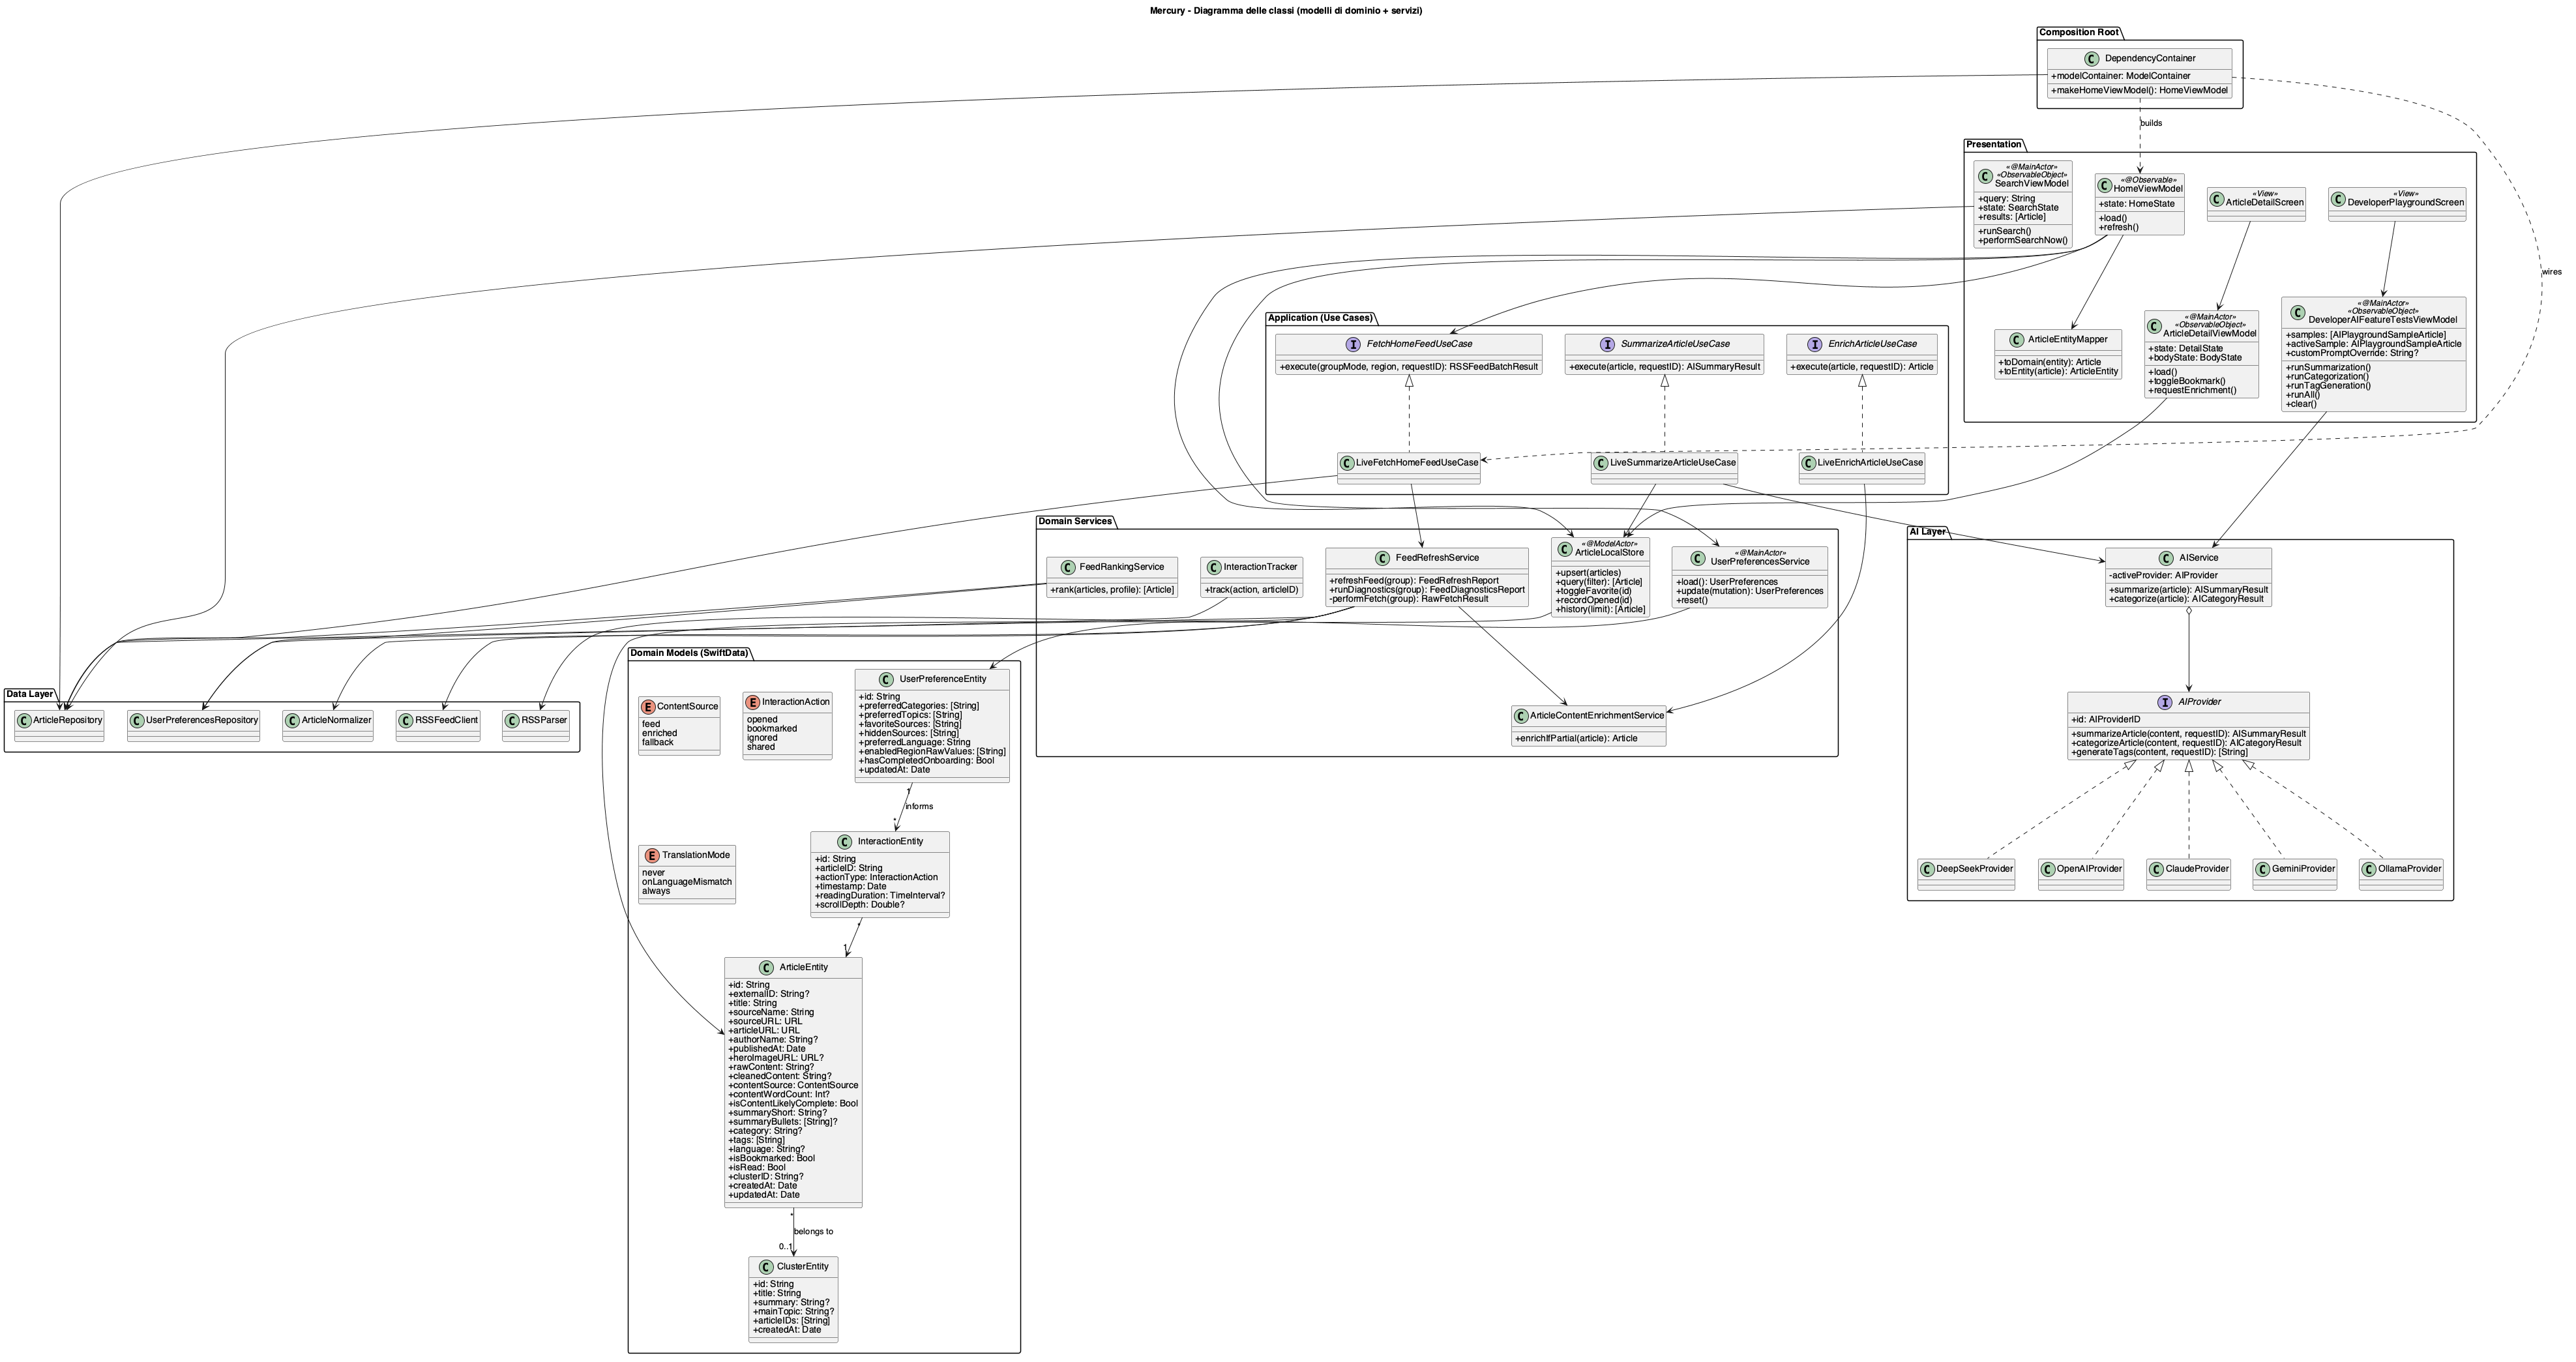
\includegraphics[width=\textwidth]{figures/class-diagram.png}
\caption{Diagramma delle classi: modelli di dominio e servizi, aggiornato allo
schema esteso post PR~\#37 con isolamento via \texttt{@ModelActor} per lo store
articoli e \texttt{@MainActor} per il servizio preferenze.}
\label{fig:class-diagram}
\end{figure}

\section{Diagrammi di sequenza}

\subsection{Ingestion RSS}
La sequenza di Fig.~\ref{fig:seq-ingestion} formalizza il flusso di refresh.
Il \texttt{HomeViewModel} attiva l'use case, che delega a
\texttt{FeedRefreshService}. Per ciascun feed si esegue fetch HTTP, parsing
RSS/Atom, normalizzazione e deduplicazione intra-feed. A valle del loop si
applica una deduplicazione cross-feed e si esegue un upsert atomico sul
repository. Ogni fallimento di fetch o parsing viene loggato e non interrompe la
pipeline; il report finale espone successi e fallimenti per outlet.

\begin{figure}[h]
\centering
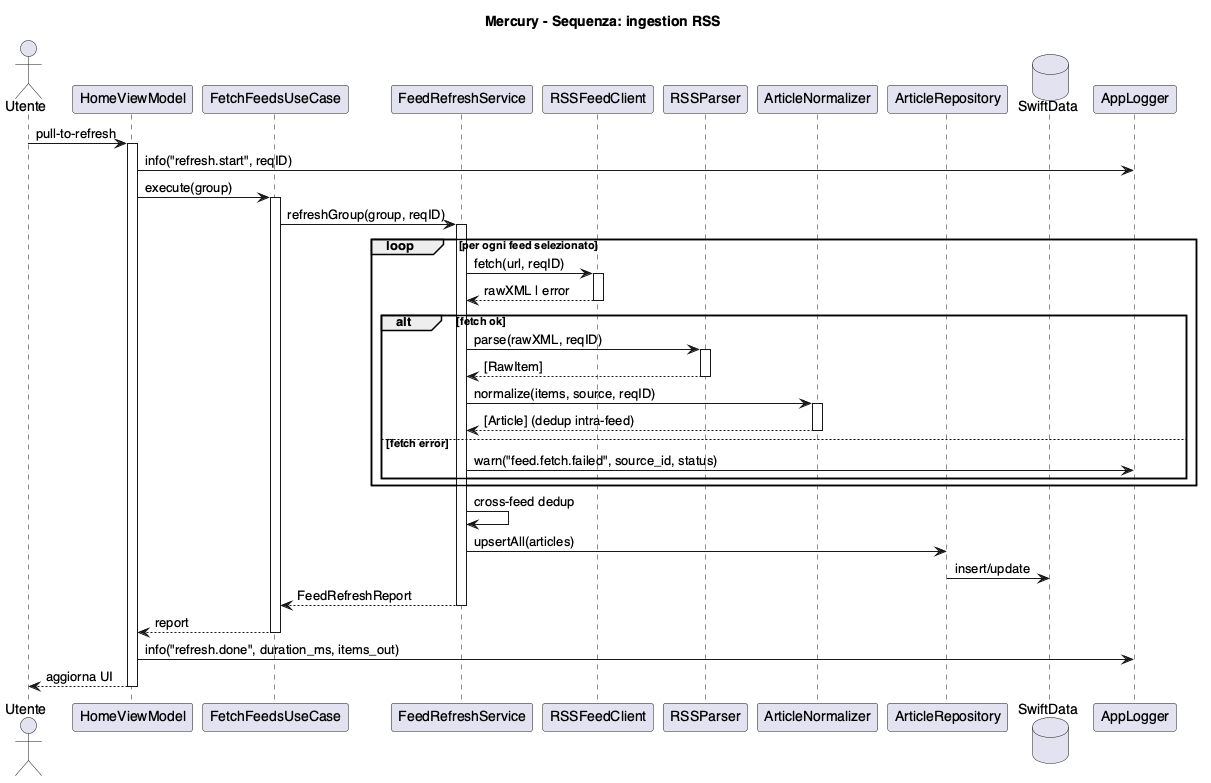
\includegraphics[width=0.95\textwidth]{figures/seq-ingestion.png}
\caption{Sequenza di ingestion RSS.}
\label{fig:seq-ingestion}
\end{figure}

\subsection{Enrichment articolo}
L'arricchimento (Fig.~\ref{fig:seq-enrichment}) è on-demand e incrementale.
Sintesi e categorizzazione possono procedere in parallelo perché operano sullo
stesso \texttt{cleanedContent} ma scrivono campi disgiunti. \texttt{AIService}
è fail-fast: in caso di errore non tenta un secondo provider, ma propaga
l'eccezione al chiamante, che decide se ritentare. Così si evitano
comportamenti sorprendenti dovuti a switch silenziosi.

\begin{figure}[h]
\centering
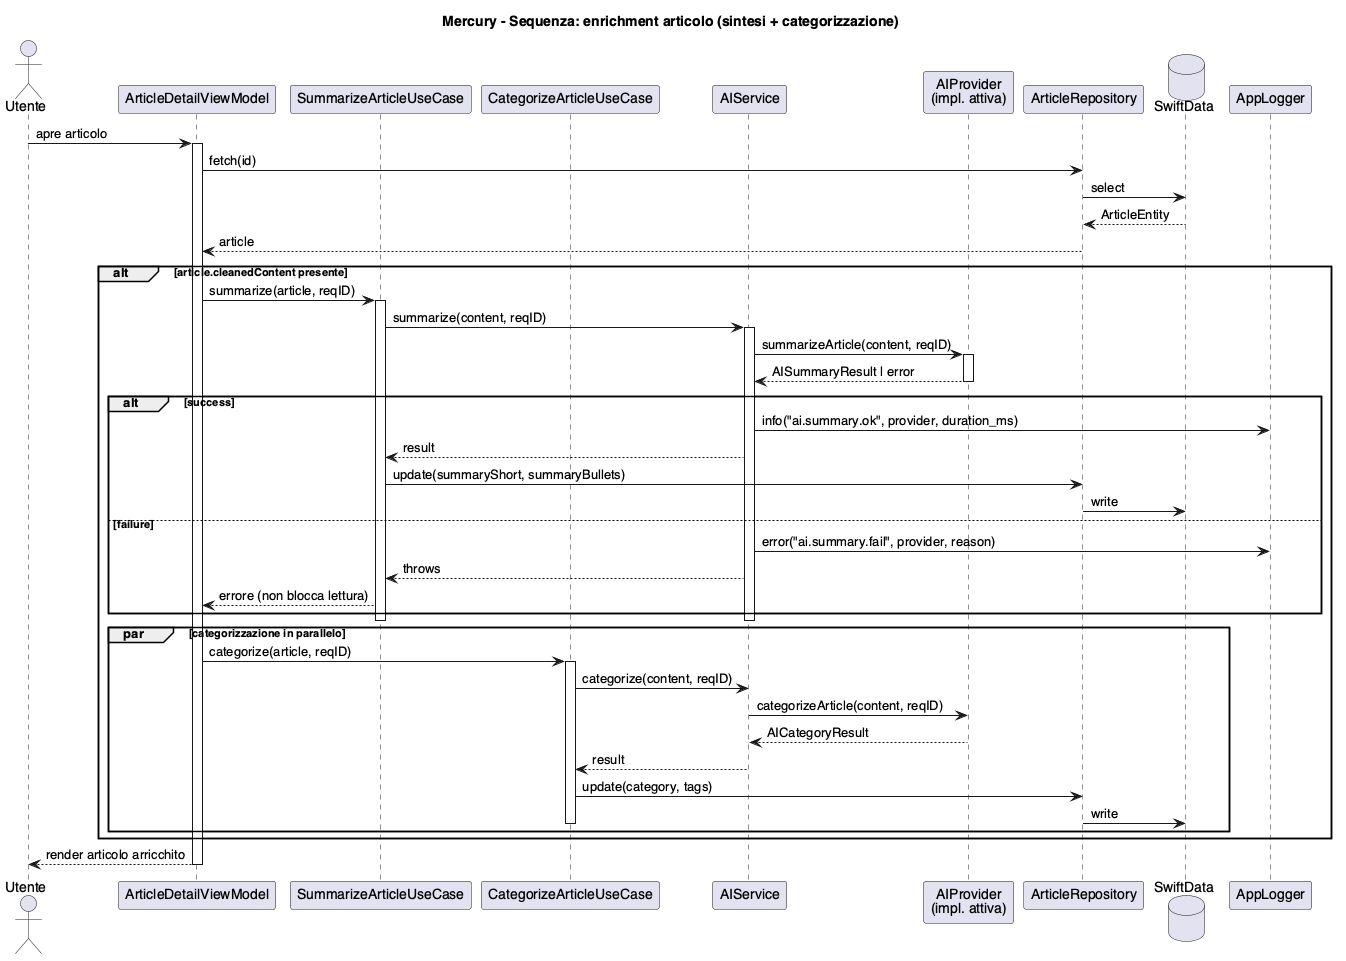
\includegraphics[width=0.95\textwidth]{figures/seq-enrichment.png}
\caption{Sequenza di enrichment di un articolo.}
\label{fig:seq-enrichment}
\end{figure}

\subsection{Ranking feed personalizzato}
La Fig.~\ref{fig:seq-ranking} descrive il flusso di costruzione del feed
personalizzato come \emph{specifica}. La specifica include il calcolo del
punteggio per articolo, controlli di diversità (evitare concentrazione su
singola fonte o micro-topic) e un fallback cronologico in caso di
insuccesso del ranking. L'implementazione la realizza in due forme: il
ranking a punteggio del feed cronologico
(sez.~\ref{sec:feed-ranking}) e il feed ``Per~te'' basato sugli
interessi dichiarati e classificato dal provider AI
(sez.~\ref{sec:personalization}); la personalizzazione sui segnali di
lettura impliciti resta specifica.

\begin{figure}[h]
\centering
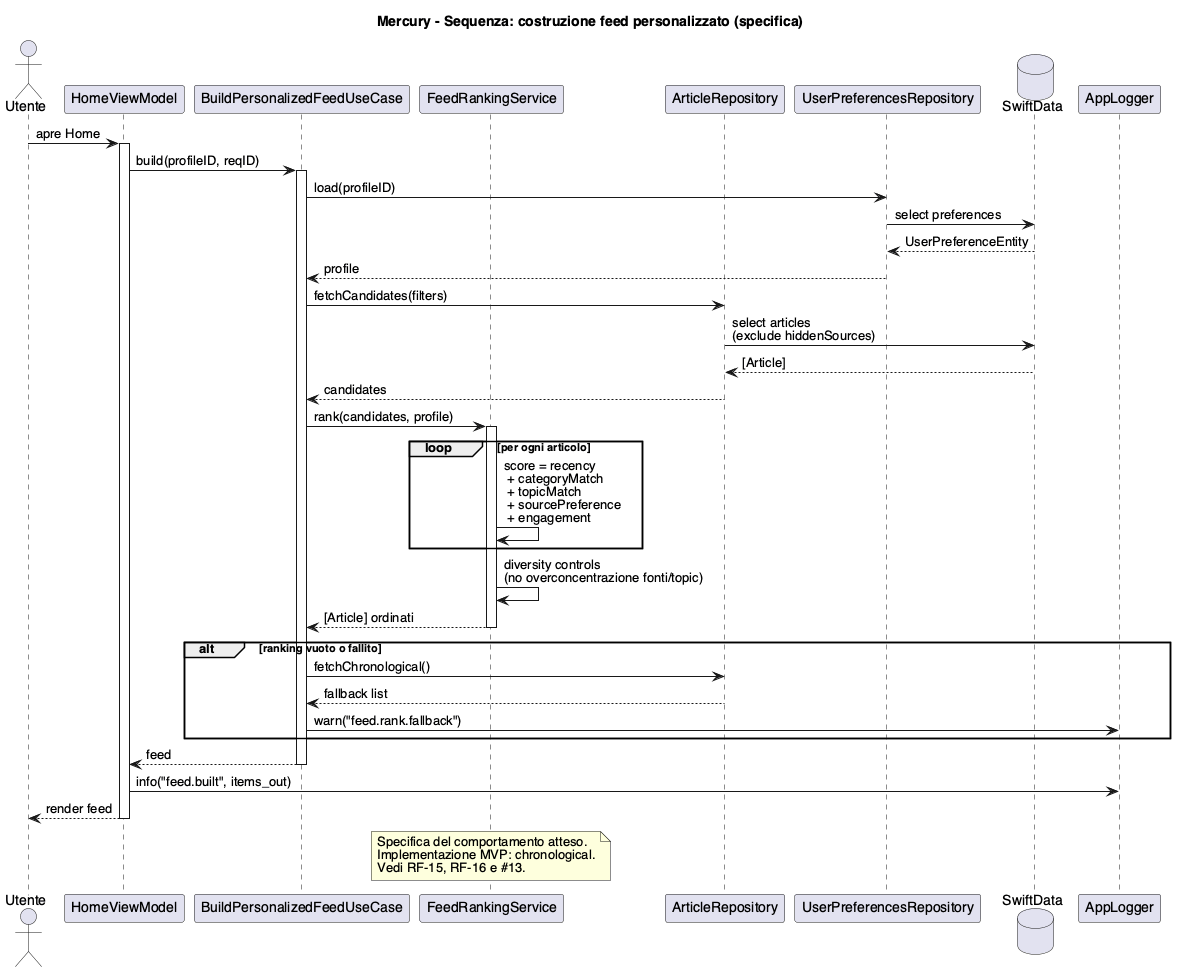
\includegraphics[width=0.95\textwidth]{figures/seq-ranking.png}
\caption{Sequenza di costruzione del feed personalizzato (specifica).}
\label{fig:seq-ranking}
\end{figure}

\subsection{Apertura dettaglio articolo}
La Fig.~\ref{fig:seq-article-detail} formalizza l'apertura del dettaglio
articolo dalla Home, realizzata in PR~\#40 (issue~\#26). Il tap sulla riga
produce una \texttt{NavigationLink} verso \texttt{ArticleDetailScreen}; il
\texttt{ArticleDetailViewModel} (\texttt{@MainActor},
\texttt{ObservableObject}) gestisce una macchina a stati
\texttt{idle}\,$\to$\,\texttt{loading}\,$\to$\,\texttt{loaded}\,$\to$\,\texttt{error}
e invoca \texttt{ArticleLocalStore} per \texttt{recordOpen} e
\texttt{toggleFavorite}. Lo slot di enrichment del corpo è una closure
iniettabile \texttt{EnrichContent?}: il servizio di sintesi AI (issue~\#28
e successive) vi è stato poi cablato senza modificare il contratto del
ViewModel, come previsto.

\begin{figure}[h]
\centering
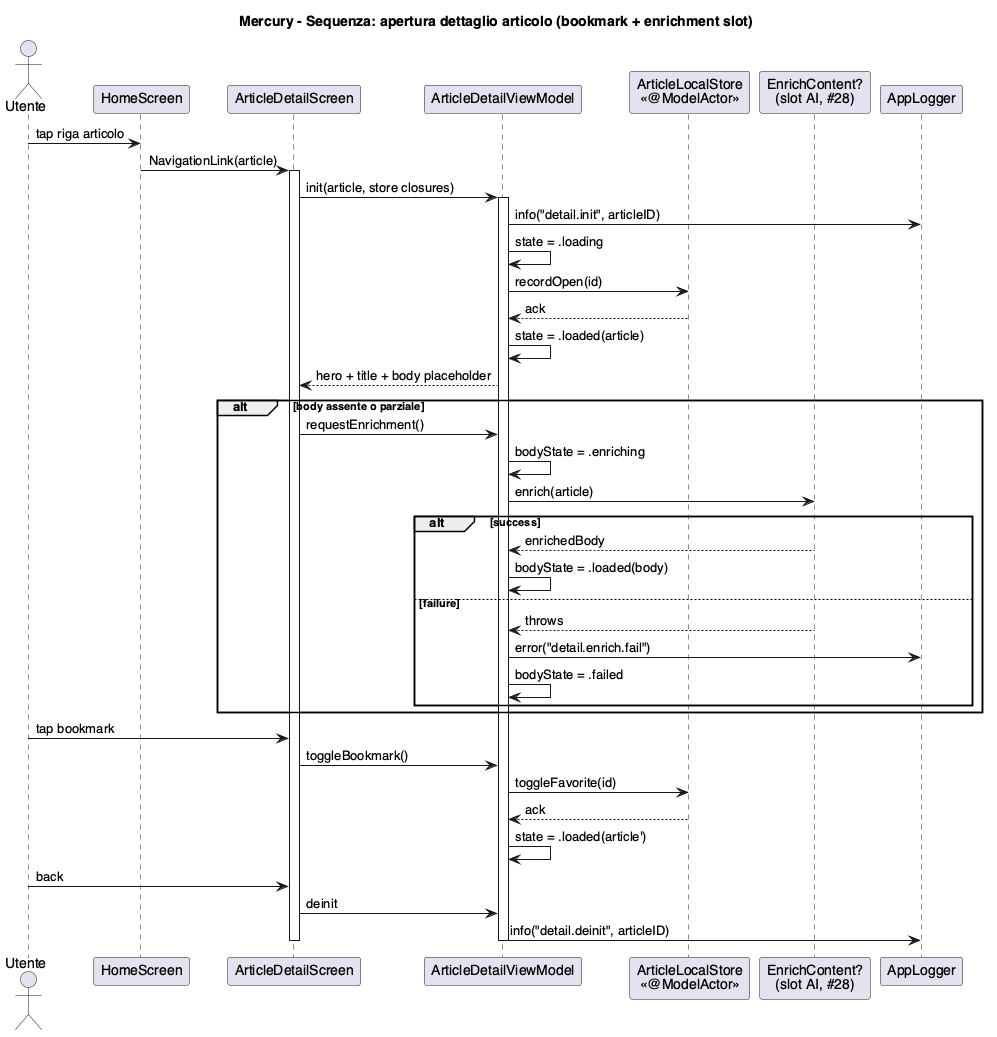
\includegraphics[width=0.95\textwidth]{figures/seq-article-detail.png}
\caption{Sequenza di apertura dettaglio articolo (PR~\#40): navigazione,
\texttt{recordOpen}, toggle bookmark e slot di enrichment.}
\label{fig:seq-article-detail}
\end{figure}

\section{Schema dati SwiftData}
La Tab.~\ref{tab:schema} sintetizza le entità persistenti e le loro relazioni.
Le chiavi primarie sono tutte \texttt{String} (UUID per profilo/interazioni,
hash URL per articoli/cluster).

\begin{table}[h]
\centering
\small
\caption{Entità SwiftData e relazioni principali.}
\label{tab:schema}
\begin{tabular}{lp{5cm}p{6cm}}
\toprule
\textbf{Entità} & \textbf{Chiave / Identità} & \textbf{Relazioni} \\
\midrule
\texttt{ArticleEntity}        & \texttt{id} = hash(\texttt{articleURL}) & \texttt{clusterID} $\to$ \texttt{ClusterEntity} (0..1) \\
\texttt{ClusterEntity}        & \texttt{id} = UUID                        & \texttt{articleIDs}: lista riferimenti \\
\texttt{UserPreferenceEntity} & \texttt{id} = UUID (singleton locale)    & --- \\
\texttt{InteractionEntity}    & \texttt{id} = UUID                       & \texttt{articleID} $\to$ \texttt{ArticleEntity} \\
\bottomrule
\end{tabular}
\end{table}

\section{Strategia di estensibilità AI}
L'astrazione \texttt{AIProvider} (Listato~\ref{lst:ai-provider}) è il punto di
estensione del layer AI. Un nuovo provider richiede:
(i)~implementare il protocollo, (ii)~registrare l'implementazione nel
\texttt{DependencyContainer}, (iii)~esporre la configurazione (modello,
timeout, endpoint) nelle preferenze sviluppatore, (iv)~aggiornare la
documentazione in \texttt{docs/ai/PROVIDERS.md}.

\begin{lstlisting}[language=Swift,label={lst:ai-provider},caption={Astrazione AIProvider (estratto, fonte \texttt{docs/architecture/ARCHITECTURE.md}).}]
protocol AIProvider {
    var id: AIProviderID { get }

    func summarizeArticle(_ content: String,
                          requestID: String?) async throws -> AISummaryResult
    func categorizeArticle(_ content: String,
                           requestID: String?) async throws -> AICategoryResult
    func generateTags(_ content: String,
                      requestID: String?) async throws -> [String]
}
\end{lstlisting}

La selezione del provider attivo avviene tramite \texttt{AIService}, che legge
le preferenze (provider id, modello, token in Keychain) e instrada le chiamate.
\texttt{AIService} non implementa fallback automatico tra provider: in caso di
errore il chiamante riceve l'eccezione e decide se ritentare o cambiare
provider esplicitamente. La scelta è documentata in
\texttt{docs/ai/PROVIDERS.md} come \emph{fail-fast by design}.

% =============================================================
\chapter{Metodologia di sviluppo agentico}
\label{cap:metodologia}

\section{Approccio e principi}
Mercury è stato sviluppato secondo un modello che chiamiamo
\emph{human-as-architect, AI-as-implementer}. All'umano spetta definire
requisiti, specifiche, scope di ogni issue, criteri di accettazione e
revisione finale. All'agente spetta tradurre l'intento in codice, nel rispetto
di una governance documentale vincolante. Il presupposto è che l'agente, se
opportunamente vincolato, sia un implementatore affidabile su task a scope
stretto, mentre l'umano resta responsabile della coerenza architetturale, della
valutazione dei trade-off e dell'integrazione nel disegno complessivo.

I principi adottati sono tre:
\begin{enumerate}
  \item \textbf{Scope ristretto per issue.} Ogni issue definisce un cambiamento
        coerente e verificabile (una feature, una correzione, una specifica).
        Le issue ``grandi'' vengono spezzate prima della delega.
  \item \textbf{Governance via documenti.} Le regole stanno nei file
        \texttt{AGENTS.md}, \texttt{docs/guidelines/CLAUDE.md},
        \texttt{docs/guidelines/CODEX.md} e \texttt{docs/guidelines/*}. Gli
        agenti li leggono come istruzioni vincolanti prima di operare.
  \item \textbf{CI come rete di sicurezza.} Build iOS, test unitari, controllo
        di sincronia tra docs e codice, lint markdown e check di localizzazione
        girano su ogni PR. Una PR rossa non viene mergiata.
\end{enumerate}

\section{Toolchain}
La toolchain di sviluppo è composta da:
\begin{itemize}
  \item \textbf{Claude Code} (Anthropic): agente CLI usato per task che
        richiedono ragionamento architetturale, refactoring multi-file e
        revisione di codice esistente;
  \item \textbf{Codex CLI} (OpenAI): agente CLI usato per task implementativi
        più diretti a scope stretto, tipicamente associati a issue numerate;
  \item \textbf{GitHub Actions}: automazione CI per build, test, lint e check
        di consistenza docs;
  \item \textbf{gh CLI}: interfaccia GitHub usata sia dagli agenti per aprire
        PR e leggere review, sia dall'umano per orchestrare il flusso.
\end{itemize}

Il criterio di scelta empirico è semplice: Codex per l'implementazione mirata su
una issue chiusa, Claude per l'analisi e il refactoring trasversale. Le branch
prodotte da Codex seguono lo schema \texttt{codex/issue-N-<slug>}, visibile
nello storico git (es.\ \texttt{codex/issue-7-swiftdata-models},
\texttt{codex/issue-21-rss-enrich}).

\section{Governance via documenti}
Il file \texttt{AGENTS.md} alla radice del repository elenca le letture
obbligatorie e le regole inderogabili. Estratto:
\begin{quote}\small\itshape
``documentation is the source of truth $\dots$ prefer the smallest coherent
change $\dots$ if behavior, contracts, models, or architecture change, update
docs in the same work session $\dots$ if new or modified functions are
introduced, add or update logs using \texttt{AppLogger}.''
\end{quote}

Il file \texttt{docs/guidelines/CODEX.md} dettaglia gli ambiti in cui un agente
può modificare il codice senza intervento umano:
\begin{quote}\small\itshape
``Codex is allowed to introduce small implementation-driven changes when
necessary $\dots$ the change must be necessary $\dots$ minimal $\dots$
consistent with the architecture $\dots$ the related docs must be updated.''
\end{quote}

La governance comprende sotto-policy specifiche e vincolanti:
\texttt{TESTING.md} (livelli di test attesi per categoria di cambiamento),
\texttt{LOCALIZATION.md} (nessuna stringa rivolta all'utente hard-coded),
\texttt{LOGGING.md} (log obbligatori in ogni funzione nuova o modificata,
propagazione del \texttt{request\_id}), \texttt{GIT\_WORKFLOW.md} (Conventional
Commits~\cite{conventionalcommits}, scope coerente, no commit a meno di
richiesta esplicita).

L'effetto pratico è che il \emph{system prompt} di ogni agente non è una
stringa magica dentro la sessione: è un insieme di file nel repository,
versionato, revisionabile e modificabile come qualunque altro artefatto di
progettazione.

\section{Flusso operativo}
Il flusso canonico è formalizzato nella Fig.~\ref{fig:seq-agentic} ed è composto
dai seguenti step:
\begin{enumerate}
  \item l'umano apre una issue su GitHub che funge da specifica (cosa,
        perché, criteri di accettazione, riferimenti ai docs);
  \item l'umano invoca un agente passando il numero della issue e indicandogli
        di leggere \texttt{AGENTS.md} e \texttt{docs/guidelines/*};
  \item l'agente crea una branch \texttt{codex/issue-N-<slug>}, esegue le
        modifiche al codice, ai test, ai log, alle stringhe localizzate e ai
        docs;
  \item l'agente apre una PR compilando il template (impatto su docs, test,
        localizzazione);
  \item la CI esegue build, test, lint e check di sincronia;
  \item l'umano effettua la review architetturale; se ok, merge;
  \item eventuali rifiniture post-merge ai docs avvengono nello stesso
        ciclo di lavoro.
\end{enumerate}

\begin{figure}[h]
\centering
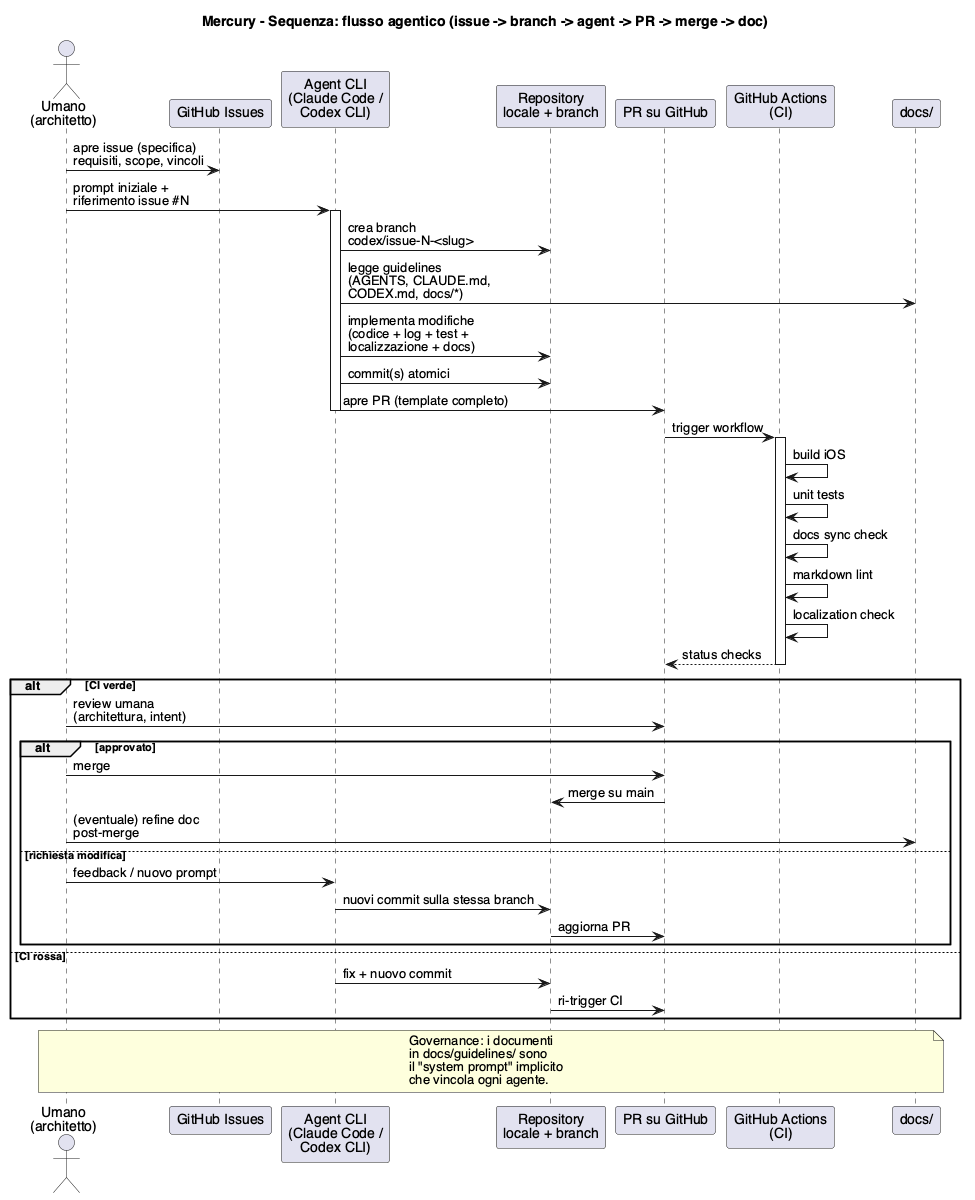
\includegraphics[width=0.95\textwidth]{figures/seq-agentic-flow.png}
\caption{Flusso agentico canonico: issue\,$\to$\,branch\,$\to$\,agent\,$\to$\,PR\,$\to$\,CI\,$\to$\,review\,$\to$\,merge.}
\label{fig:seq-agentic}
\end{figure}

\section{Pattern ricorrenti e anti-pattern}
\paragraph{Pattern che hanno funzionato.}
\begin{itemize}
  \item \emph{Issue come specifica chiusa}: più la issue è puntuale, più il
        risultato dell'agente è prevedibile (es.\ \#17 outlets export, \#18
        logging, \#7 SwiftData models).
  \item \emph{Guidelines come prompt implicito}: mettere
        \texttt{LOGGING.md} e \texttt{LOCALIZATION.md} tra le letture
        obbligatorie ha eliminato classi intere di follow-up correttivi.
  \item \emph{Doc-as-code}: la regola ``cambia comportamento $\to$ aggiorna
        docs nello stesso commit'' ha evitato il drift specifica/codice.
  \item \emph{CI scope-limited}: workflow leggeri (lint markdown, controllo
        sincronia) trovano rapidamente le incoerenze prima della review umana.
\end{itemize}

\paragraph{Anti-pattern osservati.}
\begin{itemize}
  \item \emph{Scope ambiguo}: issue formulate come ``migliorare RSS'' hanno
        prodotto modifiche fragili, che poi hanno richiesto interventi
        correttivi (cfr.\ PR~\#22 seguito dai fix \texttt{f7acbb4} e
        \texttt{8678155}).
  \item \emph{Refactor opportunistici}: tentativi di rifattorizzazioni non
        richieste dentro PR di feature; mitigati dalla regola ``no unrelated
        refactors''.
  \item \emph{Optimismo nei test}: in alcune PR i test sono stati dichiarati
        non necessari senza giustificazione; ora il template di PR li richiede
        esplicitamente.
\end{itemize}

\section{Flusso di change-request guidato dall'utente}
\label{sec:change-request}
Il flusso canonico issue\,$\to$\,branch\,$\to$\,PR descritto nella
sezione precedente copre il caso in cui la specifica è stabile e
l'implementazione segue. Il caso opposto, una \emph{change-request}
dell'utente che modifica una specifica già implementata, è gestito da una
variante distinta, formalizzata nelle linee guida di progetto. Il flusso
ha cinque step rigidi:
\begin{enumerate}
  \item \textbf{Spec change}: l'umano aggiorna i docs rilevanti
        (\texttt{docs/features/*.md}, \texttt{docs/ai/*.md},
        \texttt{docs/architecture/ARCHITECTURE.md}) come fonte di verità,
        con modifica minima e chirurgica alla sola sezione interessata;
  \item \textbf{Issue creation}: si apre una issue che linka la sezione
        docs modificata e descrive scope, anti-scope e PR eventualmente
        da revertire o correggere;
  \item \textbf{Implementation}: l'agente opera in worktree isolato con
        brief stretto, anti-scope esplicito e commit atomici;
  \item \textbf{Merge}: dopo CI verde e review, squash + delete branch.
\end{enumerate}
La regola inderogabile è ``docs prima, codice dopo'': mai modificare il
comportamento e poi i docs. Il primo esempio canonico è la modifica del
trigger di sintesi AI da automatico a on-demand, mergiata in PR~\#48
(\texttt{docs(summarization): change AI summary trigger to on-demand
button}) in $\sim$5~s con scope esclusivamente documentale (8 file
modificati, 551 inserzioni). L'issue~\#47 traccia il refactor di codice
conseguente, che resta un delta limitato perché la specifica è già
fissata nei docs.

Il contributo metodologico ha due facce. La prima: separando lo ``spec
change'' (rapido, documentale, revisionabile) dall'``implementation''
(soggetta a CI, test, review) si rende esplicito il momento in cui un
requisito è stato \emph{deciso}, distinto dal momento in cui viene
\emph{realizzato}. La seconda: il flusso evita la classe di errore più
costosa del modello agentico, cioè l'agente che reinterpreta uno scope
ambiguo durante l'implementazione. Quando la spec è già scritta sui
docs e linkata dalla issue, il margine interpretativo collassa e
l'output dell'agente diventa prevedibile.

\section{Research-as-evidence}
\label{sec:research-as-evidence}
Per i task di lavoro profondo in cui l'output non è codice ma una
\emph{base di conoscenza} (per esempio il censimento di outlet RSS, il
mapping dei provider AI, l'indagine di formati eterogenei), il flusso
canonico è stato raffinato in un pattern dedicato: il deliverable di
ricerca viene committato come \emph{artefatto JSON versionato}
\textbf{prima} che l'implementazione lo consumi. Committare l'artefatto
rende auditable la provenienza di ogni decisione successiva e disaccoppia
la fase di harvesting dalla fase di porting nel codice.

Il caso canonico è la PR~\#52 (issue~\#50), che ha esteso il catalogo
RSS a 228 outlet su 25 regioni. La fase di ricerca (Phase~A) ha
prodotto \texttt{docs/rss/research/candidates-2026-06-26.json}:
233 candidati con provenienza per outlet (URL, homepage, slant
editoriale, lingua, fonte di harvesting tra otto OPML pubblici e
registri di settore, eventuale flag \texttt{verify} per gli endpoint
fragili). L'agente di Phase~A è morto al cinquantesimo tool-use per un
rate-limit del provider, ma il JSON era già materializzato su disco:
il curatore umano lo ha committato come \texttt{b2cd647}, così che un
agente fresco di Phase~B potesse riprendere da una base stabile e
portare il catalogo nello strato Swift senza rieseguire la ricerca. Il
fallimento a metà lavoro è diventato osservabile e recuperabile in
pochi minuti, invece di un evento da contenere.

Il pattern generalizza il principio già discusso nella riflessione
sui fallimenti osservati (sez.~precedente): i checkpoint materializzati
su disco e versionati sopravvivono alla morte dell'agente. Rispetto al
normale commit incrementale cambia la natura del checkpoint, che qui
non è codice di transizione ma un deliverable di ricerca autosufficiente,
citato in seguito sia dai commit di porting (\texttt{fa1545f},
\texttt{c2f7acc}) sia dai docs per-regione (\texttt{ITALIAN\_RSS.md},
\texttt{EUROPE\_RSS.md}, \texttt{AMERICAS\_RSS.md}, \texttt{ASIA\_RSS.md})
come fonte unica di verità. La validazione effettiva degli endpoint
(Phase~3) è deferita all'issue~\#53 per non confondere lo stadio
di censimento con quello di healthcheck.

\section{Decomposizione multi-issue di una spec}
\label{sec:decomposizione-multi-issue}
Il flusso di change-request (sez.~\ref{sec:change-request}) gestisce
il caso in cui una singola modifica documentale si traduce in un solo
PR di implementazione. Serve invece una variante più articolata quando
la change-request introduce una capacità nuova che attraversa più moduli
e merita un percorso di review separato per ciascuno. Il caso canonico è
la richiesta del 30~giugno~2026 ``rendering del corpo articolo con
possibilità di scegliere tra web view e nativo'' (issue~\#51), che ha
esercitato per la prima volta il pattern.

Il flusso ha aggiunto due caratteristiche al modello a cinque step:
\begin{enumerate}
  \item \emph{Spec change documentale con scope architetturale}
        (PR~\#56): aggiornamento di tre file
        (\texttt{docs/features/ARTICLE.md} con la sezione ``Body
        Rendering'', \texttt{docs/features/SETTINGS.md} come nuovo
        feature doc, \texttt{docs/architecture/ARCHITECTURE.md} con
        il modulo §6.5). La spec ha incluso anche la
        \emph{decisione di libreria} (SwiftSoup contro Kanna/Fuzi)
        motivata dalla copertura di edge case dell'HTML reale e
        dalla licenza Apache-2.0 compatibile con il vincolo
        thesis-friendly.
  \item \emph{Decomposizione in $N$ issue} con dipendenze esplicite
        (\#57 WebView default, \#58 Settings + toggle persistito,
        \#59 renderer nativo opt-in via SwiftSoup). Ogni issue ha
        citato la sezione di docs di pertinenza come autoritativa.
  \item \emph{Stacked PR}: PR~\#60 contro \texttt{main}, PR~\#61
        contro il branch di \#60, PR~\#62 contro il branch di \#61.
        Lo stack mantiene la review per-modulo (un PR è
        verificabile in isolamento) preservando la dipendenza
        tecnica (il compilatore vede l'intera catena sul branch
        finale).
  \item \emph{Merge sequenziale con rebase automatico}: il merge di
        \#60 ha chiuso i branch dipendenti, costretto un rebase di
        \#61 su \texttt{main} (le commit di \#60 sono state
        riconosciute come già applicate dal cherry-pick detection
        di git e silenziosamente saltate), e ripetuto con \#62. La
        chiusura del chain ha richiesto la riapertura tecnica come
        PR~\#63 e \#64 dopo che GitHub ha auto-chiuso \#61 e \#62
        alla cancellazione del loro branch base. Il chain di tre PR
        è stato chiuso senza conflitti reali, perché ogni rebase ha
        solo riconosciuto contenuti identici a quelli appena
        squashati.
\end{enumerate}

Il contributo metodologico è una separazione esplicita tra
\emph{spec atomica} (una sola PR documentale, mergiabile in pochi
secondi) e \emph{implementazione segmentata} (più PR di codice,
ciascuna reviewable da un umano in pochi minuti). La somma rispetta
sia il vincolo di non accumulare PR monolitiche sia quello di
non frammentare la spec in più documenti che potrebbero divergere.
Il prezzo è la complessità del merge: il rebase automatico funziona
perché il contenuto del PR base è \emph{identico} dopo lo squash, ma
una review che richieda modifiche al PR intermedio costringe a rebase
manuali a cascata. Il pattern regge per stack di due o tre PR; oltre
quella soglia conviene una decomposizione laterale (issue indipendenti
che convergono in un solo PR di wiring).

\section{Riflessione critica}
\paragraph{Limiti.} (1)~\emph{Lock-in al tooling}: la dipendenza da agenti
commerciali (Claude, Codex) introduce un rischio di continuità in caso di
cambio di pricing o policy. Mitigazione adottata: il prompt è il repository
stesso, quindi migrabile su qualunque agente che sappia leggere
\texttt{AGENTS.md}. (2)~\emph{Allucinazioni}: gli agenti tendono a inventare
API o pattern non esistenti nel codice quando lo scope è ampio. Mitigazione:
scope ristretto e CI rigida. (3)~\emph{Debito invisibile}: gli agenti
producono codice plausibile che può accumulare debito non subito
percepibile (over-engineering, astrazioni inutili). Mitigazione: review umana
focalizzata sull'over-engineering, non solo sulla correttezza.

\paragraph{Rischi.} (1)~\emph{Drift specifica/implementazione} se il vincolo
``doc-as-code'' viene rilassato in fretta sotto pressione. (2)~\emph{Falsa
sicurezza dalla CI}: una build verde non implica che il design sia
corretto. (3)~\emph{Trasferibilità}: il modello human-as-architect richiede un
umano con competenze architetturali; non sostituisce la formazione.

\paragraph{Mitigazioni adottate.} Tutte le regole di processo sono
documentate in modo esplicito nel repository, versionate e oggetto di
review come il codice. La tracciabilità verso le issue e i PR, mantenuta
nel capitolo di metodologia e nelle tabelle dei requisiti, rende il
percorso di progetto verificabile end-to-end.

% =============================================================
\chapter{Implementazione}
\label{cap:implementazione}

Questo capitolo descrive il sistema \emph{come realizzato}, in
corrispondenza delle specifiche del Cap.~\ref{cap:specifiche} e della
progettazione del Cap.~\ref{cap:progettazione}. L'accento è sui
componenti e sulle decisioni ingegneristiche non banali; il percorso di
sviluppo (issue, revisioni, iterazioni) è discusso nel
Cap.~\ref{cap:metodologia}.

\section{Ingestione e catalogo RSS}
\label{sec:catalogo-rss}
L'ingestione è una pipeline a stadi: un client HTTP scarica i feed, un
parser RSS/Atom ne estrae i metadati estesi (titolo, link canonico,
GUID, data, lingua, autore, categorie, immagine principale, corpo), un
normalizzatore li riconduce al modello di dominio e deduplica per URL.
L'identificatore dell'articolo deriva dall'hash dell'URL, così
l'upsert è idempotente senza lookup preliminari. Il
\texttt{FeedRefreshService} espone due superfici sullo stesso core
privato: un percorso di produzione, che restituisce un report minimo
orientato al rendering, e un percorso di diagnostica, riservato al
Developer Playground, con timing e payload grezzi. Ogni errore di fetch
o parsing viene loggato e non interrompe il ciclo: il report finale
espone successi e fallimenti per singola testata.

Il catalogo delle fonti nasce come censimento multi-regione
(Tab.~\ref{tab:rss-regioni}), ma lo scope del prodotto è ristretto alle
sole testate italiane, dove si è concentrato il lavoro sulla qualità di
lettura. Le sezioni non italiane restano nel sorgente ma sono escluse
dalla compilazione tramite un flag di build
(\texttt{MERCURY\_MULTI\_REGION}): riattivarle è una modifica di una
riga, non una riscrittura. Con una sola regione l'interfaccia non mostra
alcuna selezione geografica e l'onboarding elenca direttamente le
testate italiane. In questa fase l'app assume il nome utente
\emph{Mercurio} (l'identificatore interno resta Mercury).

\begin{table}[h]
\centering
\small
\caption{Distribuzione degli outlet del censimento multi-regione.
In produzione è attiva la sola area italiana.}
\label{tab:rss-regioni}
\begin{tabular}{lr}
\toprule
\textbf{Area} & \textbf{Outlet} \\
\midrule
Italia                                             & 58 \\
Resto Europa (UK, FR, DE, ES, e altre 17 regioni)  & 138 \\
Stati Uniti                                        & 15 \\
Brasile                                            & 9 \\
Giappone                                           & 8 \\
\midrule
\textbf{Totale} su 25 regioni                      & \textbf{228} \\
\bottomrule
\end{tabular}
\end{table}

\paragraph{Validazione del catalogo.}
\label{sec:catalog-validation}
Un ``feed sano'' non è solo un feed che risponde: da ogni feed deve
essere possibile scaricare un articolo recente e ricavarne il
testo. Con questo criterio l'intero catalogo italiano è stato validato
dal vivo, rimuovendo le voci non funzionanti (archivi congelati, proxy
che restituiscono pagine senza testo, feed che servono solo la schermata
di consenso). Le poche voci degradate ma ancora utili sono annotate; il
report è mantenuto in \texttt{docs/rss/VALIDATION.md}.

\section{Persistenza locale (SwiftData)}
SwiftData~\cite{apple-swiftdata} è la sorgente di verità on-device. Le
quattro entità del Cap.~\ref{cap:specifiche} (\texttt{ArticleEntity},
\texttt{ClusterEntity}, \texttt{UserPreferenceEntity},
\texttt{InteractionEntity}) sono modelli \texttt{@Model} con mapping
da/verso il dominio. L'accesso agli articoli passa da
\texttt{ArticleLocalStore}, un \texttt{@ModelActor} che incapsula il
\texttt{ModelContext} e centralizza le invarianti (deduplica per id,
ordinamento temporale, retention), restituendo al chiamante solo tipi
valore già convertiti. Le preferenze sono gestite da
\texttt{UserPreferencesService} (\texttt{@MainActor}) con semantica di
singleton locale. Le migrazioni sono additive: i campi nuovi sono
opzionali, così aggiungere un attributo non invalida i record già
scritti.

\section{Layer AI multi-provider}
Il layer AI astrae cinque provider (OpenAI, Anthropic Claude, Google
Gemini, Ollama, DeepSeek) dietro un unico protocollo
\texttt{AIProvider}; \texttt{AIService} è l'unico punto di ingresso e
instrada le chiamate in base alle preferenze (provider, modello,
credenziali in Keychain). La scelta è \emph{fail-fast}: in caso di
errore l'eccezione risale al chiamante, senza fallback silenzioso
verso un altro provider. La deserializzazione delle risposte è
centralizzata in un unico punto, che mappa ogni anomalia di formato su
un errore tipizzato e ripara i casi ricorrenti dei modelli (JSON
troncato dal budget di token, virgole pendenti, output avvolto nel testo
di ragionamento): una sola correzione vale per tutti e cinque i
provider. Aggiungere un provider significa implementare il protocollo e
registrarlo, riusando lo scaffolding OpenAI-compatibile dove applicabile.

\section{Presentazione, orchestrazione e lettura}
La Home è governata da \texttt{HomeViewModel}, una macchina a stati
osservabile (\texttt{idle}, \texttt{loading}, \texttt{loaded},
\texttt{failed}). Il comportamento è \emph{offline-first}: all'apertura
si carica subito lo snapshot in cache e, solo se la rete è disponibile,
un refresh in background riconcilia via upsert. Tra presentazione e
servizi si interpone un layer di \emph{use case}
(\texttt{FetchHomeFeed}, \texttt{EnrichArticle},
\texttt{SummarizeArticle}) che isola la logica di dominio dai ViewModel,
coerentemente con i principi di separazione delle specifiche; ogni use
case espone un seam di test a closure, invece di introdurre un
protocollo per ogni singola dipendenza.

Il dettaglio articolo (\texttt{ArticleDetailScreen} +
\texttt{ArticleDetailViewModel}) rende corpo e metadati con una macchina
a stati e slot iniettabili per gli effetti collaterali (bookmark,
registrazione dell'apertura, arricchimento). Il corpo è reso da un
\textbf{lettore nativo} SwiftUI: l'HTML sanitizzato è parsato in blocchi
tipizzati (paragrafo, titolo, immagine, lista, citazione, codice) con
SwiftSoup~\cite{jsoup} e reso con primitive native; l'HTML malformato
ricade su un paragrafo di fallback senza generare crash. Una precedente
modalità WebView, con relativo interruttore nelle Impostazioni, è stata
rimossa a favore del solo lettore nativo: con la distillazione
(sez.~\ref{sec:distillation}) che consegna già un HTML pulito, un secondo
percorso di rendering era complessità senza beneficio.

\paragraph{Ranking del feed.}
\label{sec:feed-ranking}
Un servizio di dominio puro riordina gli articoli con uno scoring
additivo e ispezionabile a partire dalle preferenze (categoria, topic,
sorgente favorita, lingua), filtra le sorgenti nascoste e usa la
freschezza come tie-break. In assenza di segnali dell'utente diventa un
pass-through esplicito: il feed resta cronologico. Non c'è un protocollo
dietro il servizio finché esiste un solo algoritmo, per non introdurre
astrazioni speculative.

\paragraph{Ricerca locale.} La ricerca testuale opera sugli articoli in
cache con debouncing e cancellazione cooperativa. Il filtro testuale è
applicato in-memory dopo il fetch persistente, perché comporlo dentro il
\texttt{\#Predicate} di SwiftData non è affidabile; il costo è
trascurabile sul corpus dell'MVP e la scelta è isolata in un solo
metodo, reversibile quando la piattaforma lo supporterà.

\section{Lettura pulita: distillazione del corpo}
\label{sec:distillation}
Molte testate consegnano, via RSS o via pagina HTML, un corpo carico di
rumore non editoriale (banner cookie, sidebar ``Leggi anche'', strisce di
condivisione, inviti alla newsletter, immagine hero duplicata). La
distillazione è una pipeline a stadi, ispirata a Mozilla
Readability~\cite{mozilla-readability} e costruita su SwiftSoup senza
nuove dipendenze: rimozione del boilerplate per token di classe/id noti
e per densità di link; deduplicazione dell'immagine hero nel corpo;
rimozione di frasi ricorrenti localizzate (per l'italiano: ``riproduzione
riservata'', ``leggi anche'', disclaimer cookie). L'output è persistito
con un numero di versione del distillatore, così gli articoli in cache
vengono rielaborati quando la pipeline evolve; una catena di fallback
garantisce che il risultato non sia mai peggiore del testo di partenza.

\paragraph{Regole per-testata e paywall.}
\label{sec:outlet-rules-audit}
La distillazione generica non coglie il rumore specifico di ogni
testata. Un file di regole per-dominio (dati, non codice) indica per
ciascuna testata dove sta il corpo, cosa eliminare e quali frasi
rimuovere, applicato prima della distillazione generica; una regola
malformata non blocca nulla. Un classificatore di paywall riconosce gli
articoli riservati agli abbonati richiedendo \emph{due} condizioni
(testo troppo breve \emph{e} marcatore di paywall), per evitare falsi
positivi: un articolo così classificato non viene arricchito, così al
posto dell'articolo non si mostra mai il testo promozionale.

\paragraph{Stadio Readability e scorciatoia JSON-LD.}
\label{sec:readability-stage}
Poiché ogni nuovo layout richiederebbe una regola nuova, la pipeline
adotta anche Readability come stadio generico: se la pagina espone il
testo ufficiale in un blocco JSON-LD (\texttt{articleBody}), lo si usa
direttamente; altrimenti la pagina è caricata in una webview nascosta
dove Readability estrae il corpo, con fallback alla pipeline precedente
se l'estrazione rende troppo poco.

\section{Feed per argomenti e feed personalizzato}
\label{sec:topic-feed}
Oltre all'ordine cronologico, la Home offre una vista che
\emph{raggruppa per argomento} le notizie delle ultime 24 ore. Il
segnale di rilevanza è quello classico degli aggregatori: quante testate
distinte coprono la stessa storia. Il raggruppamento avviene sul
dispositivo, senza chiamate esterne: i titoli sono ridotti a vettori
TF-IDF (dopo normalizzazione e rimozione delle stopword) e confrontati
con la similarità coseno~\cite{manning2008ir}; nel dubbio si
preferisce non unire. Quando è configurato un provider AI, il
raggruppamento passa prima da lui: il modello riceve i titoli e risponde
in JSON con i gruppi, validati difensivamente, e coglie somiglianze
semantiche che il confronto lessicale non vede. Qualunque fallimento
ricade in silenzio sul clustering lessicale, così il feed non degrada
mai per colpa del provider. L'interfaccia rende esplicita l'aggregazione
(etichetta di copertura, articolo guida, sintesi AI dell'intera storia
nella lingua scelta) e la persiste per 12 ore, ricalcolandola su
trascinamento. Il clustering su embedding resta l'evoluzione prevista:
cambierebbe il vettorizzatore, non la forma della pipeline.

\subsection{Onboarding e feed ``Per te''}
\label{sec:personalization}
L'onboarding è in quattro passi: introduzione, scelta delle testate
(senza scaricare articoli), scelta degli \emph{interessi} (etichette
suggerite più campo libero) e configurazione facoltativa del provider
AI. Gli interessi alimentano il feed ``Per~te'', terzo segmento della
Home. La scelta di progetto è netta: la personalizzazione è \emph{solo
AI}, senza surrogati lessicali. Se manca il provider o mancano gli
interessi la schermata lo dichiara e rimanda alle Impostazioni, senza
mai spacciare un elenco qualunque per personalizzato. Il modello riceve
titoli e interessi e risponde con un insieme ordinato di scelte, ognuna
con l'interesse che l'ha promossa e una rilevanza; il risultato è
validato (identificatori sconosciuti e doppioni scartati) e persistito
per 12 ore, invalidato quando gli interessi cambiano. Gli interessi sono
modificabili anche dalle Impostazioni.

\section{Impostazioni, design system e osservabilità}
\paragraph{Configurazione consumer del provider AI.}
\label{sec:settings-ai}
La configurazione del provider AI, all'inizio confinata agli strumenti
sviluppatore, è promossa nelle Impostazioni: una schermata elenca i
cinque provider con lo stato (pronto / manca la chiave), attiva il
provider al tocco, accetta la chiave in un campo cifrato (mai
rimostrata), gestisce l'endpoint locale di Ollama e carica l'elenco dei
modelli. La schermata riusa un unico view model condiviso con gli
strumenti sviluppatore: un solo comportamento, due superfici.

\paragraph{Design system ``Paper''.}
\label{sec:design-system}
L'interfaccia consumer adotta un design system ispirato alla carta
stampata (sfondo carta e inchiostro adattivi al tema scuro, caratteri
con grazie per i titoli, monospazio per i metadati, filetti ed etichette
maiuscole al posto di ombre e card). I token vivono in un unico file e
la relativa guida è nella catena di lettura obbligatoria: ogni intervento
di interfaccia deve usare i token e non lo stile di default di iOS.

\paragraph{Gating dell'onboarding e cache preferenze-aware.}
\label{sec:onboarding-cache}
All'avvio l'app distingue tre stati (risposta non ancora arrivata,
onboarding da fare, completato) e non scarica nulla finché l'onboarding
non è concluso: il primo download parte solo dopo la conferma e usa
esattamente le fonti scelte. La cache è filtrata sulle preferenze (ogni
articolo porta l'identificativo della sua fonte), con pulizia immediata
degli articoli delle fonti disattivate (mai i preferiti) e retention a
30 giorni; le operazioni pesanti su SwiftData girano fuori dal main
thread per non introdurre micro-blocchi all'avvio.

\paragraph{Sintesi AI su comando.}
\label{sec:summary-button-cache}
La sintesi di un articolo è sempre esplicita, avviata da un bottone, mai
automatica all'apertura. Vale anche quando esiste una sintesi in cache,
che il tap mostra istantaneamente senza chiamare il provider. Per evitare
che l'estratto RSS venga scambiato per una sintesi AI, l'output del
modello vive in campi dedicati (\texttt{aiSummaryShort},
\texttt{aiSummaryBullets}) scritti solo dal flusso di sintesi.

\paragraph{Logging strutturato.} Ogni funzione nuova o modificata emette
log via \texttt{AppLogger} (timestamp, livello, categoria, modulo,
file/linea, funzione, request-id, metadati), con propagazione del
request-id nei flussi multi-layer; i log sono esportabili dal Developer
Playground e non contengono segreti né contenuto utente privato.

% =============================================================
\chapter{Testing e validazione}
\label{cap:testing}

\section{Strategia di test}
La strategia prevede due livelli. Gli \textbf{unit test}
(\emph{Swift Testing}) coprono modelli di dominio, use case, servizi,
repository, parser, mapper, normalizzazione delle risposte dei provider
e ViewModel; gli \textbf{UI test} (\emph{XCTest}) sono riservati ai
pochi flussi end-to-end ad alto valore (avvio, onboarding, caricamento
feed, dettaglio articolo) ed evitati per modifiche di solo layout o
copia. La regola operativa è che ogni cambiamento di comportamento
aggiorni i test al livello adeguato, oppure ne motivi esplicitamente
l'assenza.

\section{Copertura}
La copertura si concentra dove il rischio di regressione è maggiore: il
parsing RSS e la normalizzazione, la mappatura delle risposte dei
provider AI, le macchine a stati dei ViewModel e degli use case, il
ranking del feed (sez.~\ref{sec:feed-ranking}) e la pipeline di
distillazione. Quest'ultima è validata da una suite parametrica su un
corpus di pagine reali delle testate italiane, con controlli espliciti
sul contenuto che deve sopravvivere e sul chrome che deve sparire;
aggiungere una testata è un rituale documentato (nuova fixture, nuova
riga di attesa, riesecuzione della suite). Le superfici di aggregazione
e personalizzazione sono coperte da test deterministici sul clustering
lessicale, sulla validazione delle risposte AI (gruppi e scelte
personalizzate) e sulla reidratazione delle cache a 12 ore, inclusi gli
stati di assenza di provider o di interessi.

\section{Validazione qualitativa}
La validazione qualitativa si è appoggiata al Developer Playground, che
ha permesso di esercitare i parser su decine di feed reali e di isolare
classi di problemi (URL canonici incoerenti, date malformate, snippet
troncati, corpi parziali) iterando sulle euristiche di normalizzazione ed
estrazione. Lo stesso strumento isola il layer AI dal flusso consumer,
così da distinguere una regressione del provider da un problema
dell'interfaccia.

% =============================================================
\chapter{Conclusioni}
\label{cap:conclusioni}

\section{Risultati raggiunti}
Mercury raggiunge gli obiettivi MVP della tesi: una pipeline RSS robusta con
superfici separate per produzione e diagnostica (PR~\#38), una persistenza
locale-first su SwiftData con store dedicato \texttt{@ModelActor} e servizio
preferenze \texttt{@MainActor} (PR~\#34, \#35), un layer AI plug-in con
cinque provider intercambiabili (PR~\#23, \#39) reso robusto da un fix
centralizzato dell'invariante di parsing (PR~\#42), una Home
consumer-facing agganciata al feed reale (PR~\#36) e il primo flusso di
lettura completo con \texttt{ArticleDetailScreen} e slot di enrichment AI
predisposto (PR~\#40), un Developer Playground esteso con il runner
per-feature del layer AI (PR~\#41), una strumentazione di diagnostica e
logging completa, e una governance documentale che ha permesso di
sviluppare l'intero sistema con un modello human-as-architect,
AI-as-implementer. Il catalogo RSS, costruito con un artefatto di
ricerca versionato (sezione~\ref{sec:catalogo-rss}), è stato validato
dal vivo e potato a 153 feed sani
(sezione~\ref{sec:catalog-validation}). Il ciclo conclusivo sulla
qualità del lettore ha aggiunto le regole di estrazione per-outlet,
il classificatore paywall, lo stadio Readability con scorciatoia
JSON-LD e la gestione della cache
(sezioni~\ref{sec:outlet-rules-audit}, \ref{sec:readability-stage} e
\ref{sec:onboarding-cache}); coerentemente, lo scope del prodotto è
stato ristretto alle sole testate italiane e l'app rinominata
Mercurio (issue~\#102, sezione~\ref{sec:catalogo-rss}), portando lo
strato dati e l'esperienza di lettura al livello richiesto per la
demo. L'arco finale ha completato l'esperienza consumer: il design
system ``Paper'' vincolante (sez.~\ref{sec:design-system}), la Home
a tre viste con l'aggregazione per argomenti (AI col fallback
lessicale, cache di 12~ore e sintesi della storia,
sez.~\ref{sec:topic-feed}), la configurazione consumer del
provider AI (sez.~\ref{sec:settings-ai}) e l'onboarding in quattro
passi con il feed personalizzato ``Per~te'' sugli interessi
dichiarati (sez.~\ref{sec:personalization}), il tutto indurito da
quattro cicli di debugging dal vivo sul dispositivo con console
agganciata.

\section{Limiti}
La personalizzazione copre gli interessi dichiarati esplicitamente
(feed ``Per~te'', sez.~\ref{sec:personalization}) ma non ancora i
segnali di lettura impliciti (aperture, tempi di lettura, bookmark),
che restano a livello di specifica; è inoltre vincolata di proposito a
un provider AI configurato, senza surrogato locale. Il clustering è
implementato nella variante lessicale on-device con raggruppamento AI
opzionale (sez.~\ref{sec:topic-feed}), mentre la versione su embedding
resta specifica; la sincronizzazione cloud non è inclusa nell'MVP. Lo scope del
prodotto è limitato alle testate italiane (issue~\#102): è una scelta
deliberata, che concentra la qualità dove è stata misurata, ma limita la
generalità dell'app.

\section{Sviluppi futuri}
Le direzioni naturali di prosecuzione sono: (i)~estensione del feed
``Per~te'' ai segnali di lettura impliciti già modellati
(\texttt{InteractionEntity}), mantenendo il ranking ispezionabile;
(ii)~evoluzione del clustering lessicale
(sez.~\ref{sec:topic-feed}) verso embedding generati lato provider o
tramite \texttt{Natural~Language};
(iii)~sincronizzazione opzionale del profilo via Firebase; (iv)~notifiche
intelligenti basate sui topic preferiti; (v)~riattivazione del catalogo
multi-regione (già nel codice dietro il flag \texttt{MERCURY\_MULTI\_REGION}),
estendendo alle nuove testate lo stesso ciclo di audit e regole applicato a
quelle italiane.


\printbibliography[heading=bibintoc]

\end{document}
